\def\myfiledate{2022-04-22} % "\myfiledate" because packages may change \filedate
\def\thiskppversion{2.2.3}

\documentclass[twoside]{article}
\usepackage[obeyspaces]{url}
\usepackage{natbib}
\usepackage{chem}
%\usepackage{afterpage}
\usepackage{color}
\usepackage{rotating} % loads graphicx
%\usepackage{longtable}
\usepackage{graphicx}
%\usepackage{eclclass}
\usepackage{verbatim}

\oddsidemargin-5mm
\evensidemargin-15mm
\topmargin-15mm
\textheight240mm
\textwidth180mm
\raggedbottom
\parindent0mm
\parskip1.0ex plus0.5ex minus0.5ex
\renewcommand{\arraystretch}{1}
\renewcommand{\topfraction}{0.95}
\renewcommand{\dbltopfraction}{0.95}
\renewcommand{\bottomfraction}{0.95}
\renewcommand{\floatpagefraction}{0.95}
\renewcommand{\dblfloatpagefraction}{0.95}
\renewcommand{\textfraction}{0.01}
\setcounter{topnumber}{3}

\newcommand{\hhline}{\noalign{\vspace{1mm}}\hline\noalign{\vspace{1mm}}}
\newcommand{\hhlines}{\noalign{\vspace{1mm}}\hline\hline\noalign{\vspace{1mm}}}
\newcommand{\kpproot}{{\sc root}}
\newcommand{\todo}[1]{{{\color{red}\uppercase{\bf ((TODO: #1))}}}}

\def\mypageheader{Sandu \& Sander: KPP User Manual}
\markboth{\mypageheader}{\mypageheader}
\pagestyle{myheadings}

\begin{document}
\thispagestyle{empty}
\vspace*{-2cm}
\begin{center}
  {
\includegraphics[width=0.7\textwidth]{Figures/kpp-logo}}\\[9mm]
  {\Huge\bf KPP-\thiskppversion\ User's Manual}\\[9mm]
  {\huge\em The Kinetic PreProcessor KPP.}\\[5mm]
  {\huge\em An Environment for the}\\[3mm]
  {\huge\em Simulation of Chemical Kinetic Systems}\\[9mm]
  {\huge\bf Adrian Sandu$^1$ \& Rolf Sander$^2$\\[3mm]\todo{update list of authors}}\\[9mm]
  \Large
  $^1$ Department of Computer Science\\
  Virginia Polytechnic Institute and State University\\
  Blacksburg, Virginia 24060, USA\\
  \url{sandu@cs.vt.edu}\\[5mm]
  $^2$ Air Chemistry Department\\
  Max-Planck Institute of Chemistry\\
  PO Box 3060, 55020 Mainz, Germany\\
  \url{rolf.sander@mpic.de}

  \vfill

  {\large This manual is available at:
    \url{https://github.com/KineticPreProcessor/KPP/blob/main/doc/kpp_UserManual.pdf}}

\end{center}

\begin{center}
  Date: \myfiledate
\end{center}

\newpage\twocolumn

\sloppy

\tableofcontents\clearpage

%%%%%%%%%%%%%%%%%%%%%%%%%%%%%%%%%%%%%%%%%%%%%%%%%%%%%%%%%%%%%%%%%%%%%%%%%%%%%%
\section{Installation}
\label{sec:install}
%%%%%%%%%%%%%%%%%%%%%%%%%%%%%%%%%%%%%%%%%%%%%%%%%%%%%%%%%%%%%%%%%%%%%%%%%%%%%%

This section can be skipped if KPP is already installed on your system.
If you work under Linux, you can probably use the precompiled executable
file that is in the \code{bin} directory of the distribution. Then you
only have to define the \verb|$KPP_HOME| environment variable.
%
\begin{enumerate}
\item Define the \verb|$KPP_HOME| environment variable to point to the
  complete path where KPP is installed. Also, add the path of the KPP
  executable to the \verb|$PATH| environment variable. If, for example,
  KPP is installed in \verb|$HOME/kpp|, under the C shell you have to
  edit the file \verb|$HOME/.cshrc| and add:
\begin{verbatim}
setenv KPP_HOME $HOME/kpp
setenv PATH ${PATH}:$KPP_HOME/bin
\end{verbatim} %$
  If you use the bash shell, edit \code{$HOME/.bashrc} and add: %$
\begin{verbatim}
export KPP_HOME=$HOME/kpp
export PATH=$PATH:$KPP_HOME/bin
\end{verbatim} %$
  After editing \code{.cshrc} or \code{.bashrc}, start a new shell to
  make sure these changes are in effect.
\item Make sure that \code{sed} is installed on your machine. Type
  ``\code{which sed}'' to test this.
\item Make sure that \code{bison} is installed on your machine. Type
  ``\code{which bison}'' to test this.
\item Make sure that the fast lexical analyzer generator \code{flex} is
  installed on your machine. Type ``\code{flex --version}'' to test
  this. Enter the path where the flex library (\code{libfl.a} or
  \code{libfl.sh}) is located into \code{Makefile.defs}, e.g.\
  \code{FLEX_LIB_DIR=/usr/lib}.
\item Change to the KPP directory:
\begin{verbatim}
cd $KPP_HOME
\end{verbatim} %$
\item To clean the KPP installation, delete the KPP object files and all
  the examples with:
\begin{verbatim}
make clean
\end{verbatim}
To delete the KPP executable as well, type:
\begin{verbatim}
make distclean
\end{verbatim}
\item If necessary, edit \code{Makefile.defs} and enter the name of your
  C compiler. The default setting is \code{gcc}.
\item Create the kpp executable with:
\begin{verbatim}
make
\end{verbatim}
\end{enumerate}

%%%%%%%%%%%%%%%%%%%%%%%%%%%%%%%%%%%%%%%%%%%%%%%%%%%%%%%%%%%%%%%%%%%%%%%%%%%%%%
\section{Running KPP with an Example Stratospheric Mechanism}
\label{sec:model}
%%%%%%%%%%%%%%%%%%%%%%%%%%%%%%%%%%%%%%%%%%%%%%%%%%%%%%%%%%%%%%%%%%%%%%%%%%%%%%

Here we consider as an example a very simple Chapman-like mechanism for
stratospheric chemistry:
%
\begin{eqnarray}
\chem{O_2}                 & \TOHV & 2 \chem{O}\\
\chem{O} + \chem{O_2}      & \TO   & \chem{O_3}\\
\chem{O_3}                 & \TOHV & \chem{O} + \chem{O_2}\\
\chem{O} + \chem{O_3}      & \TO   & 2 \chem{O_2}\\
\chem{O_3}                 & \TOHV & \chem{O(^1D)} + \chem{O_2}\\
\chem{O(^1D)} + \chem{M}   & \TO   & \chem{O} + \chem{M}\\
\chem{O(^1D)} + \chem{O_3} & \TO   & 2 \chem{O_2}\\
\chem{NO} + \chem{O_3}     & \TO   & \chem{NO_2} + \chem{O_2}\\
\chem{NO_2} + \chem{O}     & \TO   & \chem{NO} + \chem{O_2}\\
\chem{NO_2}                & \TOHV & \chem{NO} + \chem{O}
\end{eqnarray}
%
We use the mechanism with the purpose of illustrating the KPP
capabilities. However, the software tools are general and can be applied
to virtually any kinetic mechanism.

We focus on Fortran90. Particularities of the C, Fortran77, and Matlab
languages are discussed in Sections~\ref{sec:c}, \ref{sec:f77},
\ref{sec:matlab}, respectively.

The KPP input files (with suffix \code{.kpp}) specify the model, the target
language, the precision, the integrator and the driver, etc. The file name
(without the suffix \code{.kpp}) serves as the root name for the simulation.
In this paper we will refer to this name as \kpproot. Since the root name
will be incorporated into Fortran90 module names, it can only contain
valid Fortran90 characters, i.e.\ letters, numbers, and the underscore. To
specify a KPP model, write a \kpproot\code{.kpp} file with the following
lines:
%
\begin{verbatim}
#MODEL      small_strato
#LANGUAGE   Fortran90
#DOUBLE     ON
#INTEGRATOR rosenbrock
#DRIVER     general
#JACOBIAN   SPARSE_LU_ROW
#HESSIAN    ON
#STOICMAT   ON
\end{verbatim}
%
The target language Fortran90 (i.e.\ the language of the code generated
by KPP) is selected with the command:
%
\begin{verbatim}
#LANGUAGE Fortran90
\end{verbatim}
%
Here, we have chosen Fortran90. See Sect.~\ref{sec:command-language} for
other options.

The data type of the generated model can be switched between
single/double precision with the command \code{#DOUBLE}. The
\code{#INTEGRATOR} command selects a specific numerical integration
routine (from the templates provided by KPP or implemented by the user)
and the \code{#DRIVER} command selects a specific main program. The
\code{#MODEL} command selects a specific kinetic mechanism. In our
example the model definition file \code{small_strato.def} includes the
species and the equation files,
%
\begin{verbatim}
#INCLUDE small_strato.spc
#INCLUDE small_strato.eqn
\end{verbatim}
%
The species file lists all the species in the model. Some of them are
variable (defined with \code{#DEFVAR}), meaning that their
concentrations change according to the law of mass action kinetics.
Others are fixed (defined with \code{#DEFFIX}), with the concentrations
determined by physical and not chemical factors. For each species its
atomic composition is given (unless the user chooses to ignore it). The
atom file lists the periodic table of elements in an \code{#ATOM}
section. The equation file contains the description of the equations in
an \code{#EQUATIONS} section.
%
\begin{verbatim}
#INCLUDE atoms
#DEFVAR
  O   = O;
  O1D = O;
  O3  = O + O + O;
  NO  = N + O;
  NO2 = N + O + O;
#DEFFIX
  M   = IGNORE;
  O2  = O + O;
\end{verbatim}
%
The chemical kinetic mechanism is specified in the KPP language in the
file \code{small_strato.eqn}. Each reaction is described as ``the sum of
reactants equals the sum of products'' and is followed by its rate
coefficient. \code{SUN} is the normalized sunlight intensity, equal to
one at noon and zero at night.
%
\begin{verbatim}
#EQUATIONS { Stratospheric Mechanism }
<R1>  O2  + hv = 2O       : 2.643E-10*SUN;
<R2>  O   + O2 = O3       : 8.018E-17;
<R3>  O3  + hv = O   + O2 : 6.120E-04*SUN;
<R4>  O   + O3 = 2O2      : 1.576E-15;
<R5>  O3  + hv = O1D + O2 : 1.070E-03*SUN;
<R6>  O1D + M  = O   + M  : 7.110E-11;
<R7>  O1D + O3 = 2O2      : 1.200E-10;
<R8>  NO  + O3 = NO2 + O2 : 6.062E-15;
<R9>  NO2 + O  = NO  + O2 : 1.069E-11;
<R10> NO2 + hv = NO  + O  : 1.289E-02*SUN;
\end{verbatim}
%
To run the model, type:
%
\begin{verbatim}
kpp small_strato.kpp
\end{verbatim}
%
Next, compile and run the Fortran90 code:
%
\begin{verbatim}
make -fMakefile_small_strato
./small_strato.exe
\end{verbatim}
%
%%%%%%%%%%%%%%%%%%%%%%%%%%%%%%%%%%%%%%%%%%%%%%%%%%%%%%%%%%%%%%%%%%%%%%%%%%%%%%
\section{Input for KPP}
\label{sec:input}
%%%%%%%%%%%%%%%%%%%%%%%%%%%%%%%%%%%%%%%%%%%%%%%%%%%%%%%%%%%%%%%%%%%%%%%%%%%%%%

KPP basically handles two types of files: Kinetic description files and
auxiliary files. Kinetic description files are in KPP syntax and
described in the following sections. Auxiliary files are described in
Sect.~\ref{sec:substitution-preproc}. KPP kinetic description files
specify the chemical equations, the initial values of each of the
species involved, the integration parameters, and many other options.
The KPP preprocessor parses the kinetic description files and generates
several output files. Files that are written in KPP syntax have one of
the suffixes \code{.kpp}, \code{.spc}, \code{.eqn}, or \code{.def}. An
exception is the file \code{atoms}, which has no suffix.

The following general rules define the structure of a kinetic
description file:
%
\begin{itemize}
\item A KPP program is composed of KPP sections, KPP commands and
  inlined code. Their syntax is presented in the appendix.
\item Comments are either enclosed between the curly braces ``\verb|{|''
    and ``\verb|}|'', or written in a line starting with two slashes
  ``\code{//}''.
\item Any name given by the user to denote an atom or a species is
  restricted to be less than 32 character in length and can only contain
  letters, numbers, or the underscore character. The first character
  cannot be a number. All names are case insensitive.
\end{itemize}
%
The kinetic description files contain a detailed specification of the
chemical model, information about the integration method and the desired
type of results. KPP accepts only one of these files as input, but using
the \code{#INCLUDE} command, code from separate files cn be combined.
The include files can be nested up to 10 levels. KPP will parse these
files as if they were a single big file. By carefully splitting the
chemical description, KPP can be configured for a broad range of users.
In this way the users can have direct access to that part of the model
that they are interested in, and all the other details can be hidden
inside several include files. Often, a file with atom definitions is
included first, then species definitions, and finally the equations of
the chemical mechanism.

%+++++++++++++++++++++++++++++++++++++++++++++++++++++++++++++++++++++++++++++
\subsection{KPP sections}
%+++++++++++++++++++++++++++++++++++++++++++++++++++++++++++++++++++++++++++++

\begin{table}
\begin{center}
\caption{KPP sections}
\label{tab:sections}
\begin{tabular}{lll}
\hhline
name & see Sect.\\
\hhline
\code{#ATOMS}      & \ref{sec:section-atoms}\\
\code{#CHECK}      & \ref{sec:section-check}\\
\code{#DEFFIX}     & \ref{sec:section-defvar-deffix}\\
\code{#DEFVAR}     & \ref{sec:section-defvar-deffix}\\
\code{#EQUATIONS}  & \ref{sec:section-equations}\\
\code{#INITVALUES} & \ref{sec:section-initvalues}\\
\code{#LOOKAT}     & \ref{sec:section-lookat-monitor}\\
\code{#LUMP}       & \ref{sec:section-lump}\\
\code{#MONITOR}    & \ref{sec:section-lookat-monitor}\\
\code{#SETFIX}     & \ref{sec:section-setvar-setfix}\\
\code{#SETVAR}     & \ref{sec:section-setvar-setfix}\\
\code{#TRANSPORT}  & \ref{sec:section-transport}\\
\hhline
\end{tabular}
\end{center}
\end{table}

A \code{#} sign at the beginning of a line followed by a section name
starts a new KPP section. Then a list of items separated by semicolons
follows. A section ends when another KPP section or command occurs, i.e.
when another \code{#} sign occurs at the beginning of a line. The syntax
of an item definition is different for each particular section.
Table~\ref{tab:sections} shows all the sections defined in the KPP
language. Each of them will be described separately in the following
subsections.

%-----------------------------------------------------------------------------
\subsubsection{Atom definitions ({\tt\#ATOMS})}
\label{sec:section-atoms}
%-----------------------------------------------------------------------------

The atoms that will be further used to specify the components of a
species must be declared in an \code{#ATOMS} section, e.g.:
%
\begin{verbatim}
#ATOMS N; O; Na; Br;
\end{verbatim}
%
Usually, the names of the atoms are the ones specified in the periodic
table of elements. For this table there is a predefined file containing
all definitions that can be used by the command:
%
\begin{verbatim}
#INCLUDE atoms
\end{verbatim}
%
This should be the first line in a KPP input file, because it allows to
use any atom in the periodic table of elements throughout the kinetic
description file.

%-----------------------------------------------------------------------------
\subsubsection{Mass balance checking ({\tt\#CHECK})}
\label{sec:section-check}
%-----------------------------------------------------------------------------

KPP is able to do a mass balance checking for all equations. Some
chemical equations are not balanced for all atoms, and this might still
be correct from a chemical point of view. To accommodate for this, KPP
can perform mass balance checking only for the list of atoms specified
in the \code{#CHECK} section, e.g.:
%
\begin{verbatim}
#CHECK N; C; O;
\end{verbatim}
%
The balance checking for all atoms can be enabled by using the
\code{#CHECKALL} command. Without \code{#CHECK} or \code{#CHECKALL}, no
checking is performed. The \code{IGNORE} atom can also be used to
control mass balance checking.

%-----------------------------------------------------------------------------
\subsubsection{Species definitions ({\tt\#DEFVAR} and {\tt\#DEFFIX})}
\label{sec:section-defvar-deffix}
%-----------------------------------------------------------------------------

There are two ways to declare new species together with their atom
composition: \code{#DEFVAR} and \code{#DEFFIX}. These sections define
all the species that will be used in the chemical mechanism. Species can
be variable or fixed. The type is implicitly specified by defining the
species in the appropriate sections. A species can be considered fixed
if its concentration does not vary too much. The variable species are
medium or short lived species and their concentrations vary in time.
This division of species into different categories is helpful for
integrators that benefit from treating them differently.

For each species the user has to declare the atom composition. This
information is used for mass balance checking. If the species is a
lumped species without an exact composition, it can be ignored. To do
this one can declare the predefined atom \code{IGNORE} as being part of
the species composition. Examples for these sections are:
%
\begin{verbatim}
#DEFVAR
  NO2 = N + 2O;
  CH3OOH = C + 4H + 2O;
  HSO4m = IGNORE;
  RCHO = IGNORE;
#DEFFIX
  CO2 = C + 2O;
\end{verbatim}

%-----------------------------------------------------------------------------
\subsubsection{Equations ({\tt\#EQUATIONS})}
\label{sec:section-equations}
%-----------------------------------------------------------------------------

The chemical mechanism is specified in the \code{#EQUATIONS} section.
Each equation is written in the natural way in which a chemist would
write it, e.g.:
%
\begin{verbatim}
#EQUATIONS
  NO2 + hv = NO + O : 0.533*SUN;
  OH + NO2 = HNO3 : k_3rd(temp,
    cair,2.E-30,3.,2.5E-11,0.,0.6);
\end{verbatim}
%
Only the names of already defined species can be used. The rate
coefficient has to be placed at the end of each equation, separated by a
colon. The rate coefficient does not necessarily need to be a numerical
value. Instead, it can be a valid expression in the target language. If
there are several \code{#EQUATIONS} sections in the input, their
contents will be concatenated. 

A minus sign in an equation shows that a species is consumed in a
reaction but it does not affect the reaction rate. For example, the
oxidation of methane can be written as:
%
\begin{verbatim}
CH4 + OH = CH3OO + H2O - O2 : k_CH4_OH;
\end{verbatim}
%
However, it should be noted that using negative products may lead to
numerical instabilities.

Often, the stoichiometric factors are integers. However, it is also
possible to have non-integer yields, which is very useful to
parameterize organic reactions that branch into several side reactions:
%
\begin{verbatim}
CH4 + O1D = .75 CH3O2 + .75 OH + .25 HCHO
            + .4 H + .05 H2 : k_CH4_O1D;
\end{verbatim}
%
\todo{check if the following description of prod and hv is correct}

KPP provides two pre-defined dummy species: \code{hv} and \code{PROD}.
Using dummy species does not affect the numerics of the integrators. It
only serves to improve the readability of the equations. For photolysis
reactions, \code{hv} can be specified as one of the reagents to indicate
that light ($h\nu$) is needed for this reaction, e.g.:
%
\begin{verbatim}
  NO2 + hv = NO + O : J_NO2;
\end{verbatim}
%
When the products of a reaction are not known oder not important, the
dummy species \code{PROD} should be used as a product. This is necessary
because the KPP syntax does not allow an empty list of products. For
example, the dry deposition of atmospheric ozone to the surface can be
written as:
%
\begin{verbatim}
O3 = PROD : v_d_O3;
\end{verbatim}
%
The same equation must not occur twice in the \code{#EQUATIONS} section.
For example, you may have both the gas-phase reaction of \chem{N_2O_5}
with water in your mechanism and also the heterogeneous reaction on
aerosols:
%
\begin{verbatim}
N2O5 + H2O = 2 HNO3 : k_gas;
N2O5 + H2O = 2 HNO3 : k_aerosol;
\end{verbatim}
%
These reactions must be merged by adding the rate coefficients:
%
\begin{verbatim}
N2O5 + H2O = 2 HNO3 : k_gas+k_aerosol;
\end{verbatim}

%-----------------------------------------------------------------------------
\subsubsection{Initial values ({\tt\#INITVALUES})}
\label{sec:section-initvalues}
%-----------------------------------------------------------------------------

The initial concentration values for all species can be defined in the
\code{#INITVALUES} section, e.g.:
%
\begin{verbatim}
#INITVALUES
  CFACTOR = 2.5E19;
  NO2 = 1.4E-9;
  CO2 = MyCO2Func();
  ALL_SPEC = 0.0;
\end{verbatim}
%
If no value is specified for a particular species, the default value
zero is used. One can set the default values using the generic species
names: \code{VAR_SPEC}, \code{FIX_SPEC}, and \code{ALL_SPEC}. In order
to use coherent units for concentration and rate coefficients, it is
sometimes necessary to multiply each value by a constant factor. This
factor can be set by using the generic name \code{CFACTOR}. Each of the
initial values will be multiplied by this factor before being used. If
\code{CFACTOR} is omitted, it defaults to one.

The information gathered in this section is used to generate the
\code{Initialize} subroutine (see Sect.~\ref{sec:output-init}). In more
complex 3D models, the initial values are usually taken from some input
files or some global data structures. In this case, \code{#INITVALUES}
may not be needed.

%-----------------------------------------------------------------------------
\subsubsection{Output data selection ({\tt\#LOOKAT} and {\tt\#MONITOR})}
\label{sec:section-lookat-monitor}
%-----------------------------------------------------------------------------

There are two sections in this category: \code{#LOOKAT} and
\code{#MONITOR}.

The \code{#LOOKAT} section instructs the preprocessor what are the
species for which the evolution of the concentration, should be saved in
a data file. By default, if no \code{#LOOKAT} section is present, all
the species are saved. If an atom is specified in the \code{#LOOKAT}
list then the total mass of the particular atom is reported. This allows
to check how the mass of a specific atom was conserved by the
integration method. The \code{#LOOKATALL} command can be used to specify
all the species. Output of \code{#LOOKAT} can be directed to the file
\kpproot\code{.dat} using the utility subroutines described in
Sect.~\ref{sec:output-utility}.

The \code{#MONITOR} section defines a different list of species and
atoms. This list is used by the driver to display the concentration of
the elements in the list during the integration. This may give us a
feedback of the evolution in time of the selected species during the
integration. The syntax is similar to the \code{#LOOKAT} section. With
the driver \code{general}, output of \code{#MONITOR} goes to the screen
(STDOUT). The order of the output is: first variable species, then fixes
species, finally atoms. It is not the order in the \code{#MONITOR}
command.

Examples for these sections are:
%
\begin{verbatim}
#LOOKAT NO2; CO2; O3; N;
#MONITOR O3; N;
\end{verbatim}

%-----------------------------------------------------------------------------
\subsubsection{Lump species definitions ({\tt\#LUMP})}
\label{sec:section-lump}
%-----------------------------------------------------------------------------

To reduce the stiffness of some models, various lumping of species may
be defined in the \code{#LUMP} section. The example below shows how the
concentration of \chem{NO_2} can be replaced by the sum of
concentrations for \chem{NO_2} and \chem{NO} which is considered to be a
single variable. At the end of the integration, the concentration of
\chem{NO_2} is computed by substraction from the lumped variable.
%
\begin{verbatim}
#LUMP NO2 + NO : NO2
\end{verbatim}

%-----------------------------------------------------------------------------
\subsubsection{Redefining species definitions ({\tt\#SETVAR} and
  {\tt\#SETFIX})}
\label{sec:section-setvar-setfix}
%-----------------------------------------------------------------------------

The commands \code{#SETVAR} and \code{#SETFIX} change the type of an
already defined species. Then, depending on the integration method, one
may or may not use the initial classification, or can easily move one
species from one category to another. The use of the generic species
\code{VAR_SPEC}, \code{FIX_SPEC}, and \code{ALL_SPEC} is also allowed.
Examples for these sections are:
%
\begin{verbatim}
#SETVAR ALL_SPEC;
#SETFIX H2O; CO2;
\end{verbatim}

%-----------------------------------------------------------------------------
\subsubsection{Transport ({\tt\#TRANSPORT})}
\label{sec:section-transport}
%-----------------------------------------------------------------------------

The \code{#TRANSPORT} section is only used for transport chemistry
models. It specifies the list of species that needs to be included in
the transport model, e.g.:
%
\begin{verbatim}
#TRANSPORT NO2; CO2; O3; N;
\end{verbatim}
%
One may use a more complex chemical model from which only a couple of
species are considered for the transport calculations. The
\code{#TRANSPORTALL} command is also available as a shorthand for
specifying that all the species used in the chemical model have to be
included in the transport calculations.

%+++++++++++++++++++++++++++++++++++++++++++++++++++++++++++++++++++++++++++++
\subsection{KPP commands}
%+++++++++++++++++++++++++++++++++++++++++++++++++++++++++++++++++++++++++++++

\begin{table}
\begin{center}
\caption{KPP commands}
\label{tab:commands}
\begin{tabular}{lll}
\hhline
name & see Sect.\\
\hhline
\code{#CHECKALL}     & \ref{sec:command-shorthand}\\
\code{#DECLARE}      & \ref{sec:command-declare}\\
\code{#DOUBLE}       & \ref{sec:command-double}\\
\code{#DRIVER}       & \ref{sec:command-driver}\\
\code{#DUMMYINDEX}   & \ref{sec:command-dummyindex}\\
\code{#EQNTAGS}      & \ref{sec:command-eqntags}\\
\code{#FUNCTION}     & \ref{sec:command-function}\\
\code{#HESSIAN}      & \ref{sec:command-hessian}\\
\code{#INCLUDE}      & \ref{sec:command-include}\\
\code{#INTEGRATOR}   & \ref{sec:command-integrator-intfile}\\
\code{#INTFILE}      & \ref{sec:command-integrator-intfile}\\
\code{#JACOBIAN}     & \ref{sec:command-jacobian}\\
\code{#LANGUAGE}     & \ref{sec:command-language}\\
\code{#LOOKATALL}    & \ref{sec:command-shorthand}\\
\code{#MEX}          & \ref{sec:command-mex}\\
\code{#MODEL}        & \ref{sec:command-model}\\
\code{#REORDER}      & \ref{sec:command-reorder}\\
\code{#STOCHASTIC}   & \ref{sec:command-stochastic}\\
\code{#STOICMAT}     & \ref{sec:command-stoicmat}\\
\code{#TRANSPORTALL} & \ref{sec:command-shorthand}\\
\hhline
\end{tabular}
\end{center}
\end{table}

A command begins on a new line with a \code{#} sign, followed by a
command name and one or more parameters. A summary of the commands
available in KPP is shown in Table~\ref{tab:commands}. Details about
each command are given in the following subsections.

%-----------------------------------------------------------------------------
\subsubsection{Referencing constants ({\tt\#DECLARE})}
\label{sec:command-declare}
%-----------------------------------------------------------------------------

\todo{check if this section is okay}

The \code{#DECLARE} command determines how constants like \verb|dp|,
\verb|NSPEC|, \verb|NVAR|, \verb|NFIX|, and \verb|NREACT| are inserted
into the KPP-generated code. \code{SYMBOL} (the default) means that they
are referenced by their names (e.g.\ ``C(NSPEC)''), whereas \code{VALUE}
means that their values are inserted (e.g.\ ``C(7)'').

%-----------------------------------------------------------------------------
\subsubsection{Precision control ({\tt\#DOUBLE})}
\label{sec:command-double}
%-----------------------------------------------------------------------------

The \code{#DOUBLE} command selects single or double precision
arithmetic. \code{ON} (the default) means use double precision,
\code{OFF} means use single precision (see
Sect.~\ref{sec:output-precision}).

%-----------------------------------------------------------------------------
\subsubsection{Driver selection ({\tt\#DRIVER})}
\label{sec:command-driver}
%-----------------------------------------------------------------------------

The \code{#DRIVER} command selects the driver, i.e., the file from which
the main function is to be taken. The parameter is a file name, without
suffix. The appropriate suffix (\code{.f90}, \code{.f}, \code{.c},
or \code{.m}) is automatically appended.

Normally, KPP tries to find the selected driver file in the directory
\verb|$KPP_HOME/drv/|.
However, if the supplied file name contains a slash, it is assumed to be
absolute. To access a driver in the current directory, the prefix
``\code{./}'' can be used, e.g.:
%
\begin{verbatim}
#DRIVER ./mydriver
\end{verbatim}
%
It is possible to choose the empty dummy driver \code{none}, if the user
wants to include the KPP generated modules into a larger model (e.g.\ a
general circulation or a chemical transport model) instead of creating a
stand-alone version of the chemical integrator. The driver \code{none}
is also selected when the \code{#DRIVER} command is missing. If the
\code{#DRIVER} command occurs twice, the second replaces the first.

%-----------------------------------------------------------------------------
\subsubsection{Dummy indices ({\tt\#DUMMYINDEX})}
\label{sec:command-dummyindex}
%-----------------------------------------------------------------------------

It is possible to declare species in the \code{#SPECIES} section that
are not used in the \code{#EQUATIONS} section. If your model needs to
check at run-time if a certain species is included in the current
mechanism, you can set \code{#DUMMYINDEX} to \code{ON}. Then, KPP will
set the indices \code{ind_}{\it spc} to zero for all species that do not
occur in any reaction. With \code{#DUMMYINDEX} \code{OFF} (the default),
those \code{ind_}{\it spc} are undefined variables. For example, if you
frequently switch between mechanisms with and without sulfuric acid, you
can use this code:
%
\begin{verbatim}
IF (ind_H2SO4=0) THEN
  PRINT *, 'no H2SO4 in current mechanism'
ELSE
  PRINT *, 'c(H2SO4) =', C(ind_H2SO4)
ENDIF
\end{verbatim}

%-----------------------------------------------------------------------------
\subsubsection{Generation of equation tags ({\tt\#EQNTAGS})}
\label{sec:command-eqntags}
%-----------------------------------------------------------------------------

Each reaction in the \code{#EQUATIONS} section may start with an
equation tag which is enclosed in angle brackets, e.g.:
%
\begin{verbatim}
<J1> NO2 + hv = NO + O : 0.533*SUN;
\end{verbatim}
%
With \code{#EQNTAGS} set to \code{ON}, this equation tag can be used to
refer to a specific equation, as described in
Sect.~\ref{sec:output-monitor}. The default for \code{#EQNTAGS} is
\code{OFF}.

%-----------------------------------------------------------------------------
\subsubsection{The function generation ({\tt\#FUNCTION})}
\label{sec:command-function}
%-----------------------------------------------------------------------------

The \code{#FUNCTION} command controls which functions are generated to
compute the production/destruction terms for variable species.
\code{AGGREGATE} generates one function that computes the normal
derivatives. \code{SPLIT} generates two functions for the derivatives in
production and destruction forms.

%-----------------------------------------------------------------------------
\subsubsection{Generation of Hessian ({\tt\#HESSIAN})}
\label{sec:command-hessian}
%-----------------------------------------------------------------------------

The option \code{ON} (the default) of the \code{#HESSIAN} command turns
the Hessian generation on (see Sect.~\ref{sec:output-ode-hess}). With
\code{OFF} it is switched off.

%-----------------------------------------------------------------------------
\subsubsection{File include command ({\tt\#INCLUDE})}
\label{sec:command-include}
%-----------------------------------------------------------------------------

The \code{#INCLUDE} command instructs KPP to look for the file specified
as a parameter and parse the content of this file before proceeding to
the next line. This allows the atoms definition, the species definition
and even the equation definition to be shared between several models.
Moreover this allows for custom configuration of KPP to accommodate
various classes of users. Include files can be either in one of the KPP
directories or in the current directory.

%-----------------------------------------------------------------------------
\subsubsection{Integrator selection ({\tt\#INTEGRATOR} and
  {\tt\#INTFILE})}
\label{sec:command-integrator-intfile}
%-----------------------------------------------------------------------------

The \code{#INTEGRATOR} command selects the integrator definition file.
The parameter is the file name of an integrator, without suffix. The
effect of:

\code{#INTEGRATOR} {\it integrator}

is similar to:

\code{#INCLUDE} \verb|$KPP_HOME/int/|{\it integrator}\code{.def}

The integrator definition file selects an integrator file with
\code{#INTFILE} and also defines some suitable options for it. The
\code{#INTFILE} command selects the file that contains the integrator
routine. This command allows the use of different integration techniques
on the same model. The parameter of the command is a file name, without
suffix. The appropriate suffix (\code{.f90}, \code{.f}, \code{.c}, or
\code{.m}) is appended and the result selects the file from which the
integrator is taken. This file will be copied into the code file in the
appropriate place. All integrators have to conform to the same specific
calling sequence. Normally, KPP tries to find the selected integrator
file in the directory \verb|$KPP_HOME/int/|. However, if the supplied
file name contains a slash, it is assumed to be absolute. To access an
integrator in the current directory, the prefix ``\code{./}'' can be
used, e.g.:
%
\begin{verbatim}
#INTEGRATOR ./mydeffile
#INTFILE ./myintegrator
\end{verbatim}
%
If the \code{#INTEGRATOR} command occurs twice, the second replaces the
first.

%-----------------------------------------------------------------------------
\subsubsection{The Jacobian ({\tt\#JACOBIAN})}
\label{sec:command-jacobian}
%-----------------------------------------------------------------------------

The \code{#JACOBIAN} command controls which functions are generated to
compute the Jacobian. The option \code{OFF} inhibits the generation of
the Jacobian routine. The option \code{FULL} generates the Jacobian as a
square (\code{NVAR}$\times$\code{NVAR}) matrix. It should be used if the
integrator needs the whole Jacobians. The options \code{SPARSE_ROW} and
\code{SPARSE_LU_ROW} (the default) both generate the Jacobian in sparse
(compressed on rows) format.  They should be used if the integrator
needs the whole Jacobian, but in a sparse form. The format used is
compressed on rows. With \code{SPARSE_LU_ROW}, KPP extends the number of
nonzeros to account for the fill-in due to the LU decomposition.

%-----------------------------------------------------------------------------
\subsubsection{Target language selection ({\tt\#LANGUAGE})}
\label{sec:command-language}
%-----------------------------------------------------------------------------

The \code{#LANGUAGE} command selects the target language in which the
code file is to be generated. Available options are \code{Fortran90},
\code{Fortran77}, \code{C}, or \code{Matlab}.

%-----------------------------------------------------------------------------
\subsubsection{Mex files ({\tt\#MEX})}
\label{sec:command-mex}
%-----------------------------------------------------------------------------

Mex is a \underline{m}atlab \underline{ex}tension that allows to call
functions written in Fortran and C directly from within the Matlab
environment. KPP generates the mex interface routines for the ODE
function, Jacobian, and Hessian, for the target languages C, Fortran77,
and Fortran90.  The default is \code{ON}. With \code{OFF}, no Mex files
are generated.

%-----------------------------------------------------------------------------
\subsubsection{Selcting a chemical model ({\tt\#MODEL})}
\label{sec:command-model}
%-----------------------------------------------------------------------------

The chemical model contains the description of the atoms, species, and
chemical equations. It also contains default initial values for the
species and default options including the best integrator for the model.
In the simplest case, the main kinetic description file, i.e.\ the one
passed as parameter to KPP, can contain just a single line selecting the
model. KPP tries to find a file with the name of the model and the
suffix \code{.def} in the \verb|$KPP_HOME/models| subdirectory. This
file is then parsed. The content of the model definition file is written
in the KPP language. The model definition file points to a species file
and an equation file. The species file includes further the atom
definition file. All default values regarding the model are
automatically selected. For convenience, the best integrator and driver
for the given model are also automatically selected. %$

The \code{#MODEL} command is optional, and intended for using a
predefined model. Users who supply their own reaction mechanism do not
need it.

%-----------------------------------------------------------------------------
\subsubsection{Reordering ({\tt\#REORDER})}
\label{sec:command-reorder}
%-----------------------------------------------------------------------------

Reordering of the species is performed in order to minimize the fill-in
during the LU factorization, and therefore preserve the sparsity
structure and increase efficiency.  The reordering is done using a
diagonal markowitz algorithm. The details are explained in
\citet{IMPLEMENTATION}. The default is \code{ON}. \code{OFF} means that
KPP does not reorder the species. The order of the variables is the
order in which the species are declared in the \code{#DEFVAR} section.

%-----------------------------------------------------------------------------
\subsubsection{Stochastic simulation ({\tt\#STOCHASTIC})}
\label{sec:command-stochastic}
%-----------------------------------------------------------------------------

The option \code{ON} of the \code{#STOCHASTIC} command turns on the
generation of code for stochastic kinetic simulations (see
Sect.~\ref{sec:output-stochastic}).  The default option is \code{OFF}.

%-----------------------------------------------------------------------------
\subsubsection{The Stoichiometric Formulation ({\tt\#STOICMAT})}
\label{sec:command-stoicmat}
%-----------------------------------------------------------------------------

Unless this command is set to \code{OFF}, KPP generates code for the
stoichiometric matrix, the vector of reactant products in each reaction,
and the partial derivative of the time derivative function with respect
to rate coefficients. These elements are discussed in
Sect.~\ref{sec:output-stoichiom}.

%-----------------------------------------------------------------------------
\subsubsection{Shorthand commands ({\tt\#CHECKALL}, {\tt\#LOOKATALL} and
  {\tt\#TRANSPORTALL})}
\label{sec:command-shorthand}
%-----------------------------------------------------------------------------

KPP defines a couple of shorthand commands. The commands that fall into
this category are \code{#CHECKALL}, \code{#LOOKATALL} and
\code{#TRANSPORTALL}. All of them have been described in the previous
sections.

%+++++++++++++++++++++++++++++++++++++++++++++++++++++++++++++++++++++++++++++
\subsection{Inlined code}
%+++++++++++++++++++++++++++++++++++++++++++++++++++++++++++++++++++++++++++++

In order to offer maximum flexibility, KPP allows the user to include
pieces of code in the kinetic description file. Inlined code begins on a
new line with \code{#INLINE} and the {\it inline\_type}. Next, one or
more lines of code follow, written in the target language (Fortran90,
Fortran77, C, or Matlab) as specified by the {\it inline\_type}. The
inlined code ends with \code{#ENDINLINE}. The code is inserted into the
KPP output at a position which is also determined by {\it inline\_type}
as explained in Table~\ref{tab:inlining}. If two inline commands with
the same inline type are declared, then the contents of the second is
appended to the first one. In this manual, we show the inline types for
Fortran90. The inline types for the other languages are produced by
replacing ``\code{F90_}'' by ``\code{F77_}'', ``\code{C_}'', or
``\code{MATLAB_}'', respectively.

\begin{table*}
\begin{center}
\caption{Inline types}
\vskip1mm
\label{tab:inlining}
\begin{tabular}{llll}
\hhline
{\it inline\_type} & file & placement & usage\\
\hhline
\code{F90_DATA}   & \kpproot\code{_Monitor.f90}    & specification section
                  & (obsolete)\\
\code{F90_GLOBAL} & \kpproot\code{_Global.f90}     & specification section
                  & global variables\\
\code{F90_INIT}   & \kpproot\code{_Initialize.f90} & subroutine \code{Initialize}
                  & integration parameters\\
\code{F90_RATES}  & \kpproot\code{_Rates.f90}      & executable section
                  & rate law functions\\
\code{F90_RCONST} & \kpproot\code{_Rates.f90}      & subroutine \code{UPDATE_RCONST}
                  & \code{USE} statements and definitions of rate coefficients\\
\code{F90_UTIL}   & \kpproot\code{_Util.f90}       & executable section
                  & utility functions\\
\hhline
\end{tabular}
\end{center}
\end{table*}

%-----------------------------------------------------------------------------
\subsubsection{Inline type {\tt F90\_DATA}}
\label{sec:f90-data}
%-----------------------------------------------------------------------------

This inline type was introduced in a previous version of KPP to
initialize variables. It is now obsolete but kept for compatibility. For
Fortran90, \code{F90_GLOBAL} should be used instead.

%-----------------------------------------------------------------------------
\subsubsection{Inline type {\tt F90\_GLOBAL}}
\label{sec:f90-global}
%-----------------------------------------------------------------------------

\code{F90_GLOBAL} can be used to declare global variables, e.g.\ for a
special rate coefficient:
%
\begin{verbatim}
#INLINE F90_GLOBAL
  REAL(dp) :: k_DMS_OH
#ENDINLINE
\end{verbatim}

%-----------------------------------------------------------------------------
\subsubsection{Inline type {\tt F90\_INIT}}
\label{sec:f90-init}
%-----------------------------------------------------------------------------

\code{F90_INIT} can be used to define initial values before the start of
the integartion, e.g.:
%
\begin{verbatim}
#INLINE F90_INIT
  TSTART = (12.*3600.)
  TEND = TSTART + (3.*24.*3600.)
  DT = 0.25*3600.
  TEMP = 270.
#ENDINLINE
\end{verbatim}

%-----------------------------------------------------------------------------
\subsubsection{Inline type {\tt F90\_RATES}}
\label{sec:f90-rates}
%-----------------------------------------------------------------------------

\code{F90_RATES} can be used to add new subroutines to calculate rate
coefficients, e.g.:
%
\begin{verbatim}
#INLINE F90_RATES
  REAL FUNCTION k_SIV_H2O2(k_298,tdep,cHp,temp)
    ! special rate function for S(IV) + H2O2
    REAL, INTENT(IN) :: k_298, tdep, cHp, temp
    k_SIV_H2O2 = k_298 &
      * EXP(tdep*(1./temp-3.3540E-3)) &
      * cHp / (cHp+0.1)
  END FUNCTION k_SIV_H2O2
#ENDINLINE
\end{verbatim}

%-----------------------------------------------------------------------------
\subsubsection{Inline type {\tt F90\_RCONST}}
\label{sec:f90-rconst}
%-----------------------------------------------------------------------------

\code{F90_RCONST} can be used to define time-dependent values of rate
coefficients that were declared with \code{F90_GLOBAL}:
%
\begin{verbatim}
#INLINE F90_RCONST
  k_DMS_OH = 1.E-9*EXP(5820./temp)*C(ind_O2)/ &
    (1.E30+5.*EXP(6280./temp)*C(ind_O2))
#ENDINLINE
\end{verbatim}

%-----------------------------------------------------------------------------
\subsubsection{Inline type {\tt F90\_UTIL}}
\label{sec:f90-util}
%-----------------------------------------------------------------------------

\code{F90_UTIL} can be used to define utility subroutines.

%+++++++++++++++++++++++++++++++++++++++++++++++++++++++++++++++++++++++++++++
\subsection{Auxiliary files and the substitution preprocessor}
\label{sec:substitution-preproc}
%+++++++++++++++++++++++++++++++++++++++++++++++++++++++++++++++++++++++++++++

\begin{table*}
\begin{center}
\caption{Auxiliary files (for Fortran90)}
\label{tab:aux}
\vskip4mm
%\iftwocol{\small}{}
\begin{tabular}{lll}
\hhline
File & Contents\\
\hhline
\code{dFun_dRcoeff.f90} & derivatives with respect to reaction rates\\
\code{dJac_dRcoeff.f90} & derivatives with respect to reaction rates\\
\code{Makefile.f90}     & unix makefiles\\
\code{Mex_Fun.f90}      & mex files\\
\code{Mex_Jac_SP.f90}   & mex files\\
\code{Mex_Hessian.f90}  & mex files\\
\code{sutil.f90}        & Sparse utility functions\\
\code{tag2num.f90}      & Function related to equation tags\\
\code{UpdateSun.f90}    & Function related to solar zenith angle\\
\code{UserRateLaws.f90} & User-defined rate law functions\\
\code{util.f90}         & Input/output utilities\\
\hhline
\end{tabular}
\end{center}
\end{table*}

\begin{table*}
\begin{center}
\caption{\label{tab:substitution} List of symbols replaced by the substitution
preprocessor with their particular values for the simulation at hand}
\vskip4mm
%\iftwocol{\small}{}
\begin{tabular}{lll}
\hhline
Placeholder & Replaced by & Example\\
\hhline
\code{KPP_ROOT}       & the \kpproot\ name & \code{small_strato}\\
\code{KPP_REAL}       & the real data type & \code{REAL(kind=dp)}\\
\code{KPP_NSPEC}      & number of species & 7\\
\code{KPP_NVAR}       & number of variable species & 5\\
\code{KPP_NFIX}       & number of fixed species & 2\\
\code{KPP_NREACT}     & number of chemical reactions & 10\\
\code{KPP_NONZERO}    & number of Jacobian nonzero elements & 18\\
\code{KPP_LU_NONZERO} & number of Jacobian nonzero elements, with LU fill-in & 19\\
\code{KPP_NHESS}      & number of Hessian nonzero elements & 10\\
\hhline
\end{tabular}
\end{center}
\end{table*}

The auxiliary files (listed in Table~\ref{tab:aux}) are templates for
integrators, drivers, and utilities. They are inserted into the KPP
output after being run through the substitution preprocessor. This
preprocessor replaces several placeholders (listed in
Table~\ref{tab:substitution}) in the template files with their
particular values in the model at hand. Usually, only \code{KPP_ROOT}
and \code{KPP_REAL} are needed because the other values can also be
obtained via the variables listed in Tab.~\ref{tab:parameters}.

\code{KPP_REAL} is replaced by the appropriate single or double
precision declaration type. Depending on the target language KPP will
select the correct declaration type. For example if one needs to declare
an array BIG of size 1000, a declaration like the following must be
used:

\code{KPP_REAL BIG(1000)}

When used with the option \code{#DOUBLE} \code{ON}, the above line
will be automatically translated into:

\code{REAL(dp) BIG(1000)}

and when used with the option \code{#DOUBLE} \code{OFF}, the same
line will become:

\code{REAL(sp) BIG(1000)}

in the resulting Fortran90 output file.

\code{KPP_ROOT} is replaced by the \kpproot\ file name of the main
kinetic description file. In our example where we are processing
\code{small_strato.kpp}, a line in an auxiliary Fortran90 file like
%
\begin{verbatim}
USE KPP_ROOT_Monitor
\end{verbatim}
%
will be translated into
%
\begin{verbatim}
USE small_strato_Monitor
\end{verbatim}
%
in the generated Fortran90 output file.

%%%%%%%%%%%%%%%%%%%%%%%%%%%%%%%%%%%%%%%%%%%%%%%%%%%%%%%%%%%%%%%%%%%%%%%%%%%%%%
\section{Output from KPP}
\label{sec:output}
%%%%%%%%%%%%%%%%%%%%%%%%%%%%%%%%%%%%%%%%%%%%%%%%%%%%%%%%%%%%%%%%%%%%%%%%%%%%%%

%+++++++++++++++++++++++++++++++++++++++++++++++++++++++++++++++++++++++++++++
\subsection{The Fortran90 Code}
%+++++++++++++++++++++++++++++++++++++++++++++++++++++++++++++++++++++++++++++

\begin{table*}
\begin{center}
\caption{\label{tab:generated_files} List of model files generated by
  KPP (for Fortran90). Optional files are only produced under certain
  circumstances, as specified in the third column.}
\vskip4mm
%\iftwocol{\small}{}
\begin{tabular}{llll}
\hhline
File & Description & Only if\dots & see Sect.\\
\hhline
\kpproot\code{_Main.f90}          & Driver                 & \code{#DRIVER} $\neq$ \code{none}                     & \ref{sec:output-main}       \\
\hhline
\kpproot\code{_Function.f90}      & ODE function           &                                                       & \ref{sec:output-ode-fun}    \\
\kpproot\code{_Global.f90}        & Global data headers    &                                                       & \ref{sec:output-global}     \\
\kpproot\code{_Initialize.f90}    & Initialization         &                                                       & \ref{sec:output-init}       \\
\kpproot\code{_Integrator.f90}    & Numerical integration  &                                                       & \ref{sec:output-integrator} \\
\kpproot\code{_LinearAlgebra.f90} & Sparse linear algebra  &                                                       & \ref{sec:output-la}         \\
\kpproot\code{_Model.f90}         & Summary of modules     &                                                       & \ref{sec:output-model}      \\
\kpproot\code{_Monitor.f90}       & Equation info          &                                                       & \ref{sec:output-monitor}    \\
\kpproot\code{_Parameters.f90}    & Model parameters       &                                                       & \ref{sec:output-parameters} \\
\kpproot\code{_Precision.f90}     & Parameterized types    &                                                       & \ref{sec:output-precision}  \\
\kpproot\code{_Rates.f90}         & User-defined rate laws &                                                       & \ref{sec:output-rates}      \\
\kpproot\code{_Util.f90}          & Utility input-output   &                                                       & \ref{sec:output-utility}    \\
\hhline
\kpproot\code{_Jacobian.f90}      & ODE Jacobian           &                                                       & \ref{sec:output-ode-jac}    \\
\kpproot\code{_JacobianSP.f90}    & Jacobian sparsity      & \code{#JACOBIAN SPARSE_}$*$                           & \ref{sec:output-ode-jac}    \\
\hhline
\kpproot\code{_Hessian.f90}       & ODE Hessian            & \code{#HESSIAN ON}                                    & \ref{sec:output-ode-hess}   \\
\kpproot\code{_HessianSP.f90}     & Sparse Hessian data    & \code{#HESSIAN ON} and \code{#JACOBIAN SPARSE_}$*$    & \ref{sec:output-ode-hess}   \\
\hhline
\kpproot\code{_Stochastic.f90}    & Stochastic functions   & \code{#STOCHASTIC ON}                                 & \ref{sec:output-stochastic} \\
\hhline
\kpproot\code{_Stoichiom.f90}     & Stoichiometric model   & \code{#STOICMAT ON}                                   & \ref{sec:output-stoichiom}  \\
\kpproot\code{_StoichiomSP.f90}   & Stoichiometric matrix  & \code{#STOICMAT ON} and \code{#JACOBIAN SPARSE_}$*$   & \ref{sec:output-stoichiom}  \\
\hhline
\kpproot\code{_mex_Fun.f90}       & Matlab interface Fun   & \code{#MEX ON}                                        & \ref{sec:output-mexcode}    \\
\kpproot\code{_mex_Jac_SP.f90}    & Matlab interface Jac   & \code{#MEX ON} and \code{#JACOBIAN SPARSE_}$*$        & \ref{sec:output-mexcode}    \\
\kpproot\code{_mex_Hessian.f90}   & Matlab interface Hess  & \code{#MEX ON} and \code{#HESSIAN ON}                 & \ref{sec:output-mexcode}    \\
\hhline
\code{Makefile_}\kpproot          & Makefile               &                                                       & \ref{sec:output-makefile}   \\
\hhline
\kpproot\code{.map}               & Human-readable info    &                                                       & \ref{sec:output-map}        \\
\hhline
\end{tabular}
\end{center}
\end{table*}

\begin{figure*}[htbp]
  \centering
  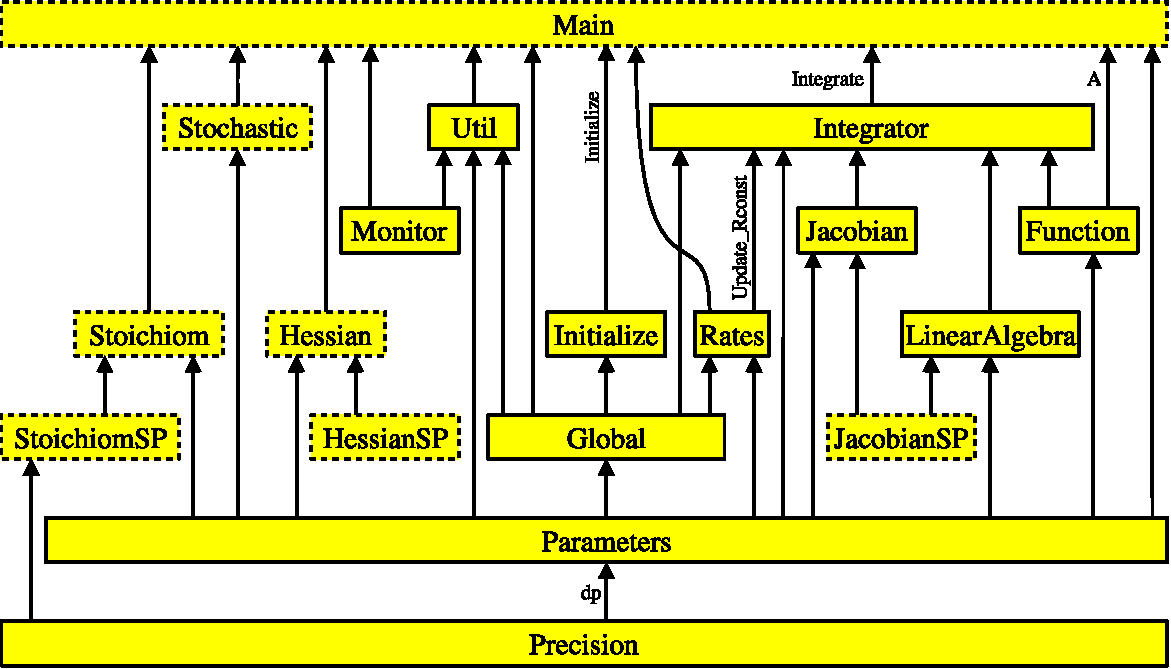
\includegraphics[width=\textwidth]{Figures/kpp2_use_diagr}
  \caption{Interdependencies of the KPP-generated
    files. Each arrow starts at the module that exports a variable or
    subroutine and points to the module that imports it via the
    Fortran90 USE instruction. The prefix \texttt{\kpproot\_} has been
    omitted from the module names for better readability. Dotted boxes
    show optional files that are only produced under certain
    circumstances, as listed in Tab.~\ref{tab:generated_files}.}
  \label{fig:use_diagr}
\end{figure*}

\begin{table*}
\begin{center}
\caption{\label{tab:functions} List of selected Fortran90 subroutines
  generated by KPP}
\vskip4mm
%\iftwocol{\small}{}
\begin{tabular}{lll}
\hhline
Subroutine              & Description                                 & File\\
\hhline
\code{Fun}              & ODE function                                & \kpproot\code{_Function.f90}\\
\hhline
\code{Jac_SP}           & ODE Jacobian in sparse format               & \kpproot\code{_Jacobian.f90}\\
\code{Jac_SP_Vec}       & sparse multiplication                       & \kpproot\code{_Jacobian.f90}\\
\code{JacTR_SP_Vec}     & sparse multiplication                       & \kpproot\code{_Jacobian.f90}\\
\code{Jac}              & ODE Jacobian in full format                 & \kpproot\code{_Jacobian.f90}\\
\hhline
\code{Hessian}          & ODE Hessian in sparse format                & \kpproot\code{_Hessian.f90}\\
\code{Hess_Vec}         & Hessian action on vectors                   & \kpproot\code{_Hessian.f90}\\
\code{HessTR_Vec}       & Transposed Hessian action on vectors        & \kpproot\code{_Hessian.f90}\\
\hhline
\code{dFun_dRcoeff}     & Derivatives of Fun with respect to rate coefficients & \kpproot\code{_Stoichiom.f90}\\
\code{dJac_dRcoeff}     & Derivatives of Jac with respect to rate coefficients & \kpproot\code{_Stoichiom.f90}\\
\code{ReactantProd}     & Reactant products                           & \kpproot\code{_Stoichiom.f90}\\
\code{JacReactantProd}  & Jacobian of reactant products               & \kpproot\code{_Stoichiom.f90}\\
\hhline
\code{KppDecomp}        & Sparse LU decomposition                     & \kpproot\code{_LinearAlgebra.f90}\\
\code{KppSolve}         & Sparse back substitution                    & \kpproot\code{_LinearAlgebra.f90}\\
\hhline
\code{Update_PHOTO}     & Update photolysis rate coefficients         & \kpproot\code{_Rates.f90}\\
\code{Update_RCONST}    & Update all rate coefficients                & \kpproot\code{_Rates.f90}\\
\code{Update_SUN}       & Update solar intensity                      & \kpproot\code{_Rates.f90}\\
\hhline
\code{Initialize}       & Set initial values                          & \kpproot\code{_Initialize.f90}\\
\hhline
\code{Integrate}        & Integrate one time step                     & \kpproot\code{_Integrator.f90}\\
\hhline
\code{GetMass}          & Check mass balance for selected atoms       & \kpproot\code{_Util.f90}\\
\code{Shuffle_kpp2user} & Shuffle concentration vector                & \kpproot\code{_Util.f90}\\
\code{Shuffle_user2kpp} & Shuffle concentration vector                & \kpproot\code{_Util.f90}\\
\code{InitSaveData}     & Utility for \code{#LOOKAT} command          & \kpproot\code{_Util.f90}\\
\code{SaveData}         & Utility for \code{#LOOKAT} command          & \kpproot\code{_Util.f90}\\
\code{CloseSaveData}    & Utility for \code{#LOOKAT} command          & \kpproot\code{_Util.f90}\\
\code{tag2num}          & Calculate reaction number from equation tag & \kpproot\code{_Util.f90}\\
\hhline
\end{tabular}
\end{center}
\end{table*}

The code generated by KPP is organized in a set of separate files. Each
has a time stamp and a complete description of how it was generated at
the begining of the file. The files associated with \kpproot\ are named
with a corresponding prefix ``\kpproot\code{_}''. The list of files and
a short description is shown in Table~\ref{tab:generated_files}. All
subroutines and functions, global parameters, variables, and sparsity
data structures are encapsulated in modules. There is exactly one module
in each file, and the name of the module is identical to the file name
but without the suffix \code{.f90}. Fig.~\ref{fig:use_diagr} shows how
these modules are related to each other. A concise list of the main
subroutines generated by KPP is shown in Table~\ref{tab:functions}. The
generated code is consistent with the Fortran90 standard. It will not
exceed the maximum number of 39 continuation lines. If KPP cannot
properly split an expression to keep the number of continuation lines
below the threshold then it will generate a warning message pointing to
the location of this expression.

%-----------------------------------------------------------------------------
\subsubsection{\kpproot{\tt\_Main.f90}}
\label{sec:output-main}
%-----------------------------------------------------------------------------

\kpproot\code{_Main.f90} is the main Fortran90 program. It contains the
driver after modifications by the substitution preprocessor. The name of
the file is computed by KPP by appending the suffix \code{_Main.f90}
to the \kpproot\ name.

%-----------------------------------------------------------------------------
\subsubsection{\kpproot{\tt\_Model.f90}}
\label{sec:output-model}
%-----------------------------------------------------------------------------

The file \kpproot{\tt\_Model.f90} completely defines the model by using
all the associated modules.

%-----------------------------------------------------------------------------
\subsubsection{\kpproot{\tt\_Initialize.f90}}
\label{sec:output-init}
%-----------------------------------------------------------------------------

The file \kpproot{\tt\_Initialize.f90} contains the subroutine \code{Initialize}
which defines initial values of the chemical species. The driver calls
the subroutine \code{Initialize} once before the time integration loop
starts.

%-----------------------------------------------------------------------------
\subsubsection{\kpproot{\tt\_Integrator.f90}}
\label{sec:output-integrator}
%-----------------------------------------------------------------------------

The file \kpproot{\tt\_Integrator.f90} contains the subroutine
\code{INTEGRATE} which is called every time step during the integration.
The integrator that was chosen with \code{#INTEGRATOR} is also included
in \kpproot{\tt\_Integrator.f90}. In case of an unsuccessful
integration, the module \kpproot\code{_Integrator} provides a short
error message in the public variable \code{IERR_NAME}.

%-----------------------------------------------------------------------------
\subsubsection{\kpproot{\tt\_Monitor.f90}}
\label{sec:output-monitor}
%-----------------------------------------------------------------------------

The file \kpproot{\tt\_Monitor.f90} contains \code{PARAMETER} arrays
with information about the chemical mechanism. The names of all species
are included in \code{SPC_NAMES} and the names of all equations are
included in \code{EQN_NAMES}.

It was shown above (Sect.~\ref{sec:command-eqntags}) that each reaction
in the \code{#EQUATIONS} section may start with an equation tag which is
enclosed in angle brackets, e.g.:
%
\begin{verbatim}
<J1> NO2 + hv = NO + O : 0.533*SUN;
\end{verbatim}
%
If the equation tags are switched on, KPP also generates the
\code{PARAMETER} array \code{EQN_TAGS}. In combination with
\code{EQN_NAMES} and the function \code{tag2num} that converts the
equation tag to the KPP-internal equation number, this can be used to
describe a reaction:
%
\begin{verbatim}
  PRINT *,'Reaction J1 is:', &
    EQN_NAMES(tag2num('J1'))
\end{verbatim}

%-----------------------------------------------------------------------------
\subsubsection{\kpproot{\tt\_Precision.f90}}
\label{sec:output-precision}
%-----------------------------------------------------------------------------

Fortran90 code uses parameterized real types.
\kpproot\code{_Precision.f90} contains the following real kind
definitions:
%
\begin{verbatim}
! KPP_SP - Single precision kind
  INTEGER, PARAMETER :: &
    SP = SELECTED_REAL_KIND(6,30)
! KPP_DP - Double precision kind
  INTEGER, PARAMETER :: &
    DP = SELECTED_REAL_KIND(12,300)
\end{verbatim}
%
Depending on the choice of the \code{#DOUBLE} command, the real
variables are of type double (\code{REAL(kind=R_8)}) or single precision
(\code{REAL(kind=R_4)}). Changing the parameters of the
\code{SELECTED_REAL_KIND} function in this module will cause a change in
the working precision for the whole model.

%-----------------------------------------------------------------------------
\subsubsection{\kpproot{\tt\_Rates.f90}}
\label{sec:output-rates}
%-----------------------------------------------------------------------------

The code to update the rate constants is in \kpproot\code{_Rates.f90}.
The user defined rate law functions are also placed here.

%-----------------------------------------------------------------------------
\subsubsection{\kpproot{\tt\_Parameters.f90}}
\label{sec:output-parameters}
%-----------------------------------------------------------------------------

The global parameters (Table~\ref{tab:parameters}) are defined and
initialized in \kpproot\code{_Parameters.f90}.

KPP orders the variable species such that the sparsity pattern of the
Jacobian is maintained after an LU decomposition. For our
\code{small_strato} example there are five variable species
(\code{NVAR}=5) ordered as
%
\begin{verbatim}
ind_O1D=1, ind_O=2, ind_O3=3,
ind_NO=4, ind_NO2=5
\end{verbatim}
%
and two fixed species (\code{NFIX}=2)
%
\begin{verbatim}
ind_M = 6, ind_O2 = 7.
\end{verbatim}
%
KPP defines a complete set of simulation parameters, including the numbers
of variable and fixed species, the number of chemical reactions, the
number of nonzero entries in the sparse Jacobian and in the sparse
Hessian, etc. Some important simulation parameters generated by KPP are
presented in Table~\ref{tab:parameters}.

\begin{table}
\caption{\label{tab:parameters} List of important simulation parameters
  and their values for the {\tt small\_strato} example}
\vskip4mm
%\iftwocol{\small}{}
\begin{tabular}{ll@{}r}
\hhline
Parameter & Represents & Value\\
\hhline
\code{NSPEC}          & No. chemical species                             &  7\\
\code{NVAR}           & No. variable species                             &  5\\
\code{NFIX}           & No. fixed species                                &  2\\
\code{NREACT}         & No. reactions                                    & 10\\
\code{NONZERO}        & No. nonzero entries Jacobian                     & 18\\
\code{LU_NONZERO}     & As above, after LU factorization                 & 19\\
\code{NHESS}          & Length, sparse Hessian                           & 10\\
\code{NJVRP}          & Length, sparse Jacobian \code{JVRP}              & 13\\
\code{NSTOICM}        & Length, stoichiometric matrix                    & 22\\
\code{ind_}{\it spc}  & Index of species {\it spc} in \code{C()}         &\\
\code{indf_}{\it spc} & Index of fixed species {\it spc} in \code{FIX()} &\\
\hhline
\end{tabular}
\end{table}

%-----------------------------------------------------------------------------
\subsubsection{\kpproot{\tt\_Global.f90}}
\label{sec:output-global}
%-----------------------------------------------------------------------------

The global variables (Table~\ref{tab:global}) are declared in
\kpproot\code{_Global.f90}. Global variables are presented in
Table~\ref{tab:global}.

\begin{table}
\caption{\label{tab:global} List of important global variables}
\vskip4mm
%\iftwocol{\small}{}
\begin{tabular}{ll}
\hhline
Global variable & Represents\\
\hhline
\code{C(NSPEC)}          & Concentrations, all species\\
\code{VAR(NVAR)}         & Concentrations, variable species\\
\code{FIX(NFIX)}         & Concentrations, fixed species\\
\code{RCONST(NREACT)}    & Rate coefficient values\\
\code{TIME}              & Current integration time\\
\code{SUN}               & Sun intensity between 0 and 1\\
\code{TEMP}              & Temperature\\
\code{TSTART,TEND}       & Simulation start/end time\\
\code{DT}                & Simulation step\\
\code{ATOL(NSPEC)}       & Absolute tolerances\\
\code{RTOL(NSPEC)}       & Relative tolerances\\
\code{STEPMIN}           & Lower bound for time step\\
\code{STEPMAX}           & Upper bound for time step\\
\code{CFACTOR}           & Conversion factor\\
\code{SPC_NAMES(NSPEC)}  & Names of chemical species\\
\code{EQN_NAMES(NREACT)} & Names of chemical equations\\
\hhline
\end{tabular}
\end{table}

Both variable and fixed species are stored in the one-dimensional array
\code{C}. The first part (indices from 1 to \code{NVAR}) contains the
variable species, and the second part (indices from \code{NVAR+1} to
\code{NSPEC}) the fixed species. The total number of species
\code{NSPEC} is the sum of the \code{NVAR} and \code{NFIX}. The parts
can also be accessed separately through the arrays \code{VAR} and
\code{FIX}:
%
\begin{verbatim}
VAR(1:NVAR) = C(1:NVAR)
FIX(1:NFIX) = C(NVAR+1:NSPEC)
\end{verbatim}

%-----------------------------------------------------------------------------
\subsubsection{\kpproot{\tt\_Function.f90}}
\label{sec:output-ode-fun}
%-----------------------------------------------------------------------------

The chemical ODE system for our example is:
%
\def\dd{{\mathrm{d}}}
\begin{eqnarray*}
  \frac{\dd\, [\chem{O(^1D)}]}{\dd t} & = & k_{5}\, [\chem{O_3}] - k_{6}\,
  [\chem{O(^1D)}]\, [\chem{M}] - k_{7}\, [\chem{O(^1D)}]\, [\chem{O_3}]\\
  \frac{\dd\, [\chem{O}]}{\dd t} & = & 2\, k_{1}\, [\chem{O_2}] - k_{2}\,
  [\chem{O}]\, [\chem{O_2}] + k_{3}\, [\chem{O_3}]\\
  & & - k_{4}\, [\chem{O}]\, [\chem{O_3}]+ k_{6}\, [\chem{O(^1D)}]\,
  [\chem{M}]\\
  & & - k_{9}\, [\chem{O}]\, [\chem{NO_2}] + k_{10}\, [\chem{NO_2}]\\
  \frac{\dd\, [\chem{O_3}]}{\dd t} & = & k_{2}\, [\chem{O}]\, [\chem{O_2}] -
  k_{3}\, [\chem{O_3}] - k_{4}\, [\chem{O}]\, [\chem{O_3}] - k_{5}\,
  [\chem{O_3}]\\
  & & - k_{7}\, [\chem{O(^1D)}]\, [\chem{O_3}] - k_{8}\, [\chem{O_3}]\, 
  [\chem{NO}]\\
  \frac{\dd\, [\chem{NO}]}{\dd t} & = & - k_{8}\, [\chem{O_3}]\, [\chem{NO}] +
  k_{9}\, [\chem{O}]\, [\chem{NO_2}] + k_{10}\, [\chem{NO_2}]\\
  \frac{\dd\, [\chem{NO_2}]}{\dd t} & = & k_{8}\, [\chem{O_3}]\, [\chem{NO}] -
  k_{9}\, [\chem{O}]\, [\chem{NO_2}] - k_{10}\, [\chem{NO_2}]
\end{eqnarray*}
%
where square brackets denote concentrations of the species. The code for
the ODE function is in \kpproot\code{_Function.f90}. The chemical
reaction mechanism represents a set of ordinary differential equations
(ODEs) of dimension \code{NVAR}. The concentrations of fixed species are
parameters in the derivative function. The subroutine \code{Fun}
computes first the vector \code{A} of reaction rates and then the vector
\code{Vdot} of variable species time derivatives. The input arguments
\code{V}, \code{F}, and \code{RCT} are the concentrations of variable
species, fixed species, and the rate coefficients, respectively. Below
is the Fortran90 code generated by KPP for the ODE function of our
\code{small_strato} example.
%
\begin{verbatim}
SUBROUTINE Fun (V, F, RCT, Vdot )
   REAL(kind=DP) ::  V(NVAR), &
         F(NFIX), RCT(NREACT), &
         Vdot(NVAR), A(NREACT) &
! Computation of equation rates
   A(1) = RCT(1)*F(2)
   A(2) = RCT(2)*V(2)*F(2)
   A(3) = RCT(3)*V(3)
   A(4) = RCT(4)*V(2)*V(3)
   A(5) = RCT(5)*V(3)
   A(6) = RCT(6)*V(1)*F(1)
   A(7) = RCT(7)*V(1)*V(3)
   A(8) = RCT(8)*V(3)*V(4)
   A(9) = RCT(9)*V(2)*V(5)
   A(10) = RCT(10)*V(5)
! Aggregate function
   Vdot(1) = A(5)-A(6)-A(7)
   Vdot(2) = 2*A(1)-A(2)+A(3) &
             -A(4)+A(6)-A(9)+A(10)
   Vdot(3) = A(2)-A(3)-A(4)-A(5) &
             -A(7)-A(8)
   Vdot(4) = -A(8)+A(9)+A(10)
   Vdot(5) = A(8)-A(9)-A(10)
END SUBROUTINE Fun
\end{verbatim}

%-----------------------------------------------------------------------------
\subsubsection{\kpproot{\tt\_Jacobian.f90} and \kpproot{\tt\_JacobianSP.f90}}
\label{sec:output-ode-jac}
%-----------------------------------------------------------------------------

\begin{figure}[htbp]
  \centering
  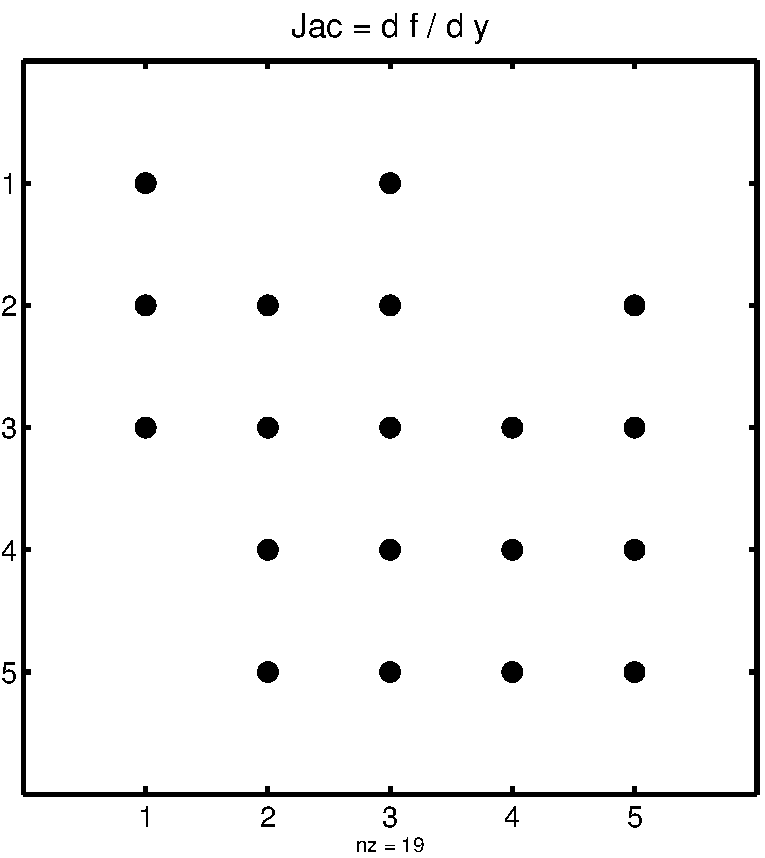
\includegraphics[width=0.8\columnwidth]{Figures/small_jac}
  \caption{The sparsity pattern of the Jacobian for the {\tt
      small\_strato} example. All non-zero elements are marked with a
    bullet. Note that even though {\tt J(3,5)=0}, it is also included
    here because of the fill-in. \todo{Adrian, is this explanation of
      J(3,5) correct?}}
  \label{fig:jac}
\end{figure}

The Jacobian matrix for our example contains 18 non-zero elements:

\begin{eqnarray*}
  \mathbf{J}(1,1) & = & - k_{6}\, [\chem{M}] - k_{7}\, [\chem{O_3}]\\
  \mathbf{J}(1,3) & = & k_{5} - k_{7}\, [\chem{O(^1D)}]\\
  \mathbf{J}(2,1) & = & k_{6}\, [\chem{M}]\\
  \mathbf{J}(2,2) & = & - k_{2}\, [\chem{O_2}] - k_{4}\, [\chem{O_3}] 
                        - k_{9}\, [\chem{NO_2}]\\
  \mathbf{J}(2,3) & = & k_{3} - k_{4}\, [\chem{O}]\\
  \mathbf{J}(2,5) & = & - k_{9}\, [\chem{O}] + k_{10}\\
  \mathbf{J}(3,1) & = & - k_{7}\, [\chem{O_3}]\\
  \mathbf{J}(3,2) & = & k_{2}\, [\chem{O_2}] - k_{4}\, [\chem{O_3}]\\
  \mathbf{J}(3,3) & = & - k_{3} - k_{4}\, [\chem{O}] - k_{5} - k_{7}\, 
                        [\chem{O(^1D)}] - k_{8}\, [\chem{NO}]\\
  \mathbf{J}(3,4) & = & - k_{8}\, [\chem{O_3}]\\
  \mathbf{J}(4,2) & = & k_{9}\, [\chem{NO_2}]\\
  \mathbf{J}(4,3) & = & - k_{8}\, [\chem{NO}]\\
  \mathbf{J}(4,4) & = & - k_{8}\, [\chem{O_3}]\\
  \mathbf{J}(4,5) & = & k_{9}\, [\chem{O}] + k_{10}\\
  \mathbf{J}(5,2) & = & - k_{9}\, [\chem{NO_2}]\\
  \mathbf{J}(5,3) & = & k_{8}\, [\chem{NO}]\\
  \mathbf{J}(5,4) & = & k_{8}\, [\chem{O_3}]\\
  \mathbf{J}(5,5) & = & - k_{9}\, [\chem{O}] - k_{10}\\
\end{eqnarray*}

It defines how the temporal change of each chemical species depends on
all other species. For example, $\mathbf{J}(5,2)$ shows that \chem{NO_2}
(species number 5) is affected by \chem{O} (species number 2) via
reaction number R9. The sparse data structures for the Jacobian are
declared and initialized in \kpproot\code{_JacobianSP.f90}. The code for
the ODE Jacobian and sparse multiplications is in
\kpproot\code{_Jacobian.f90}. The Jacobian of the ODE function is
automatically constructed by KPP. KPP generates the Jacobian subroutine
\code{Jac} or \code{Jac_SP} where the latter is generated when the
sparse format is required. Using the variable species \code{V}, the
fixed species \code{F}, and the rate coefficients \code{RCT} as input,
the subroutine calculates the Jacobian \code{JVS}. The default data
structures for the sparse compressed on rows Jacobian representation are
shown in Table~\ref{tab:sparse-jac} (for the case where the LU fill-in
is accounted for). \code{JVS} stores the \code{LU_NONZERO} elements of
the Jacobian in row order. Each row \code{I} starts at position
\code{LU_CROW(I)}, and \code{LU_CROW(NVAR+1)=LU_NONZERO+1}. The location
of the \code{I}-th diagonal element is \code{LU_DIAG(I)}. The sparse
element \code{JVS(K)} is the Jacobian entry in row \code{LU_IROW(K)} and
column \code{LU_ICOL(K)}. For the \code{small_strato} example KPP
generates the following Jacobian sparse data structure:
%
\begin{verbatim}
LU_ICOL = (/ 1,3,1,2,3,5,1,2,3,4, &
            5,2,3,4,5,2,3,4,5 /)
LU_IROW = (/ 1,1,2,2,2,2,3,3,3,3, &
            3,4,4,4,4,5,5,5,5 /)
LU_CROW = (/ 1,3,7,12,16,20 /)
LU_DIAG = (/ 1,4,9,14,19,20 /)
\end{verbatim}
%
This is visualized in Fig.~\ref{fig:jac}. The sparsity coordinate
vectors are computed by KPP and initialized statically. These vectors
are constant as the sparsity pattern of the Jacobian does not change
during the computation.

\begin{table}
\caption{\label{tab:sparse-jac} Sparse Jacobian Data Structures}
\vskip4mm
%\iftwocol{\small}{}
\begin{tabular}{ll}
\hhline
Global variable & Represents\\
\hhline
\code{JVS(LU_NONZERO)}     & Jacobian nonzero elements\\
\code{LU_IROW(LU_NONZERO)} & Row indices\\
\code{LU_ICOL(LU_NONZERO)} & Column indices\\
\code{LU_CROW(NVAR+1)}     & Start of rows\\
\code{LU_DIAG(NVAR+1)}     & Diagonal entries\\
\hhline
\end{tabular}
\end{table}

Two other KPP-generated routines, \code{Jac_SP_Vec} and
\code{JacTR_SP_Vec} are useful for direct and adjoint sensitivity
analysis. They perform sparse multiplication of \code{JVS} (or its
transpose for \code{JacTR_SP_Vec}) with the user-supplied vector
\code{UV} without any indirect addressing.

%-----------------------------------------------------------------------------
\subsubsection{\kpproot{\tt\_Hessian.f90} and \kpproot{\tt\_HessianSP.f90}}
\label{sec:output-ode-hess}
%-----------------------------------------------------------------------------

\begin{figure*}[htbp]
  \centering 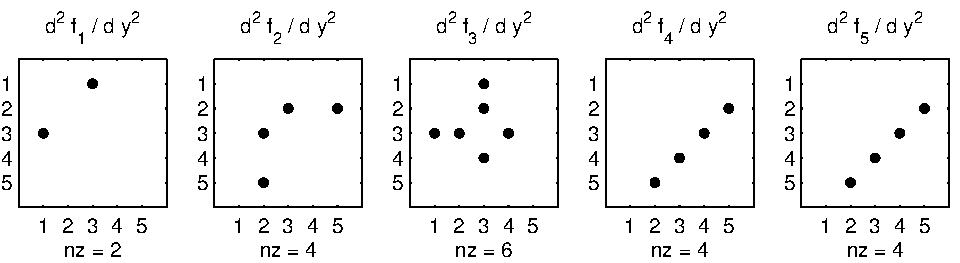
\includegraphics[width=0.8\textwidth]{Figures/small_hess1}
  \caption{The Hessian of the {\tt small\_strato} example.}
  \label{fig:hess1}
\end{figure*}

The sparse data structures for the Hessian are declared and initialized
in \kpproot\code{_HessianSP.f90}. The Hessian function and associated
sparse multiplications are in \kpproot\code{_Hessian.f90}. The Hessian
contains the second order derivatives of the time derivative functions.
More exactly, the Hessian is a 3-tensor such that
%
\begin{equation}
H_{i,j,k} = \frac{\partial^2 (\dd c/\dd t)_i}{\partial c_j \,\partial c_k}~,
  \qquad 1 \le i,j,k \le N_{\rm var}~.
\label{eqn:Hessian1}
\end{equation}
%
KPP generates the routine \code{Hessian}. Using the variable species
\code{V}, the fixed species \code{F}, and the rate coefficients
\code{RCT} as input, the subroutine calculates the Hessian. The Hessian
is a very sparse tensor. The sparsity of the Hessian for our
\code{small_strato} example is visualized in Fig.~\ref{fig:hess1}. KPP
computes the number of nonzero Hessian entries and saves it in the
variable \code{NHESS}. The Hessian itself is represented in coordinate
sparse format. The real vector \code{HESS} holds the values, and the
integer vectors \code{IHESS_I}, \code{IHESS_J}, and \code{IHESS_K} hold
the indices of nonzero entries as illustrated in
Table~\ref{tab:sparse-hess}. Since the time derivative function is
smooth, these Hessian matrices are symmetric,
\code{HESS}$_{i,j,k}$=\code{HESS}$_{i,k,j}$. KPP stores only those
entries \code{HESS}$_{i,j,k}$ with $j \le k$. The sparsity coordinate
vectors \code{IHESS_I}, \code{IHESS_J}, and \code{IHESS_K} are computed
by KPP and initialized statically. They are constant as the sparsity
pattern of the Hessian does not change during the computation.

\begin{table}
\caption{\label{tab:sparse-hess} Sparse Hessian Data}
\vskip4mm
%\iftwocol{\small}{}
\begin{tabular}{ll}
\hhline
Variable & Represents\\
\hhline
\code{HESS(NHESS)}    & Hessian nonzero elements \code{H}$_{i,j,k}$\\
\code{IHESS_I(NHESS)} & Index $i$ of element \code{H}$_{i,j,k}$\\
\code{IHESS_J(NHESS)} & Index $j$ of element \code{H}$_{i,j,k}$\\
\code{IHESS_K(NHESS)} & Index $k$ of element \code{H}$_{i,j,k}$\\
\hhline
\end{tabular}
\end{table}

The routines \code{Hess_Vec} and \code{HessTR_Vec} compute the action of
the Hessian (or its transpose) on a pair of user-supplied vectors
\code{U1} and \code{U2}. Sparse operations are employed to produce the
result vector.

%-----------------------------------------------------------------------------
\subsubsection{\kpproot{\tt\_LinearAlgebra.f90}}
\label{sec:output-la}
%-----------------------------------------------------------------------------

Sparse linear algebra routines are in the file
\kpproot\code{_LinearAlgebra.f90}. To numerically solve for the chemical
concentrations one must employ an implicit timestepping technique, as
the system is usually stiff. Implicit integrators solve systems of the
form
%
\begin{equation}
P\, x = (I - h \gamma J)\, x = b
\end{equation}
%
where the matrix $P=I - h \gamma J$ is refered to as the ``prediction
matrix''. $I$ the identity matrix, $h$ the integration time step,
$\gamma$ a scalar parameter depending on the method, and $J$ the system
Jacobian. The vector $b$ is the system right hand side and the solution
$x$ typically represents an increment to update the solution.

The chemical Jacobians are typically sparse, i.e.\ only a relatively
small number of entries are nonzero. The sparsity structure of $P$ is
given by the sparsity structure of the Jacobian, and is produced by KPP
(with account for the fill-in) as discussed above.

KPP generates the sparse linear algebra subroutine \code{KppDecomp}
which performs an in-place, non-pivoting, sparse LU decomposition of the
prediction matrix $P$. Since the sparsity structure accounts for
fill-in, all elements of the full LU decomposition are actually stored.
The output argument \code{IER} returns a value that is nonzero if
singularity is detected.

The subroutines \code{KppSolve} and \code{KppSolveTR} use the in-place
LU factorization $P$ as computed by \code{KppDecomp} and perform sparse
backward and forward substitutions (using $P$ or its transpose). The
sparse linear algebra routines \code{KppDecomp} and \code{KppSolve} are
extremely efficient, as shown by \citep{IMPLEMENTATION}.

%-----------------------------------------------------------------------------
\subsubsection{\kpproot{\tt\_Stoichiom.f90} and \kpproot{\tt\_StoichiomSP.f90}}
\label{sec:output-stoichiom}
%-----------------------------------------------------------------------------

These files contain a description of the chemical mechanism in
stoichiometric form. The file \kpproot\code{_Stoichiom.f90} contains the
functions for reactant products and its Jacobian, and derivatives with
respect to rate coefficients. The declaration and initialization of the
stoichiometric matrix and the associated sparse data structures is done
in \kpproot\code{_StoichiomSP.f90}.

The stoichiometric matrix is constant sparse. For our example the matrix
has \code{NSTOICM=}22 nonzero entries out of 50 entries. KPP produces
the stoichiometric matrix in sparse, column-compressed format, as shown
in Table~\ref{tab:sparse-stoicm}. Elements are stored in columnwise
order in the one-dimensional vector of values \code{STOICM}. Their row
and column indices are stored in \code{IROW_STOICM} and
\code{ICOL_STOICM} respectively. The vector \code{CCOL_STOICM} contains
pointers to the start of each column. For example column \code{j} starts
in the sparse vector at position \code{CCOL_STOICM(j)} and ends at
\code{CCOL_STOICM(j+1)-1}. The last value
\code{CCOL_STOICM(NVAR+1)=NSTOICM+1} simplifies the handling of sparse
data structures.

\begin{table}
\caption{\label{tab:sparse-stoicm} Sparse Stoichiometric Matrix}
\vskip4mm
%\iftwocol{\small}{}
\begin{tabular}{ll}
\hhline
Global variable & Represents\\
\hhline
\code{STOICM(NSTOICM)}       & Stoichiometric matrix\\
\code{IROW_STOICM(NSTOICM)}  & Row indices\\
\code{ICOL_STOICM(NSTOICM)}  & Column indices\\
\code{CCOL_STOICM(NREACT+1)} & Start of columns\\
\hhline
\end{tabular}
\end{table}

The subroutine \code{ReactantProd} computes the reactant products
\code{ARP} for each reaction, and the subroutine \code{JacReactantProd}
computes the Jacobian of reactant products vector, i.e.:
%
\begin{equation}
{\tt JVRP} = \partial {\tt ARP} / \partial {\tt V}
\end{equation}
%
The matrix \code{JVRP} is sparse and is computed and stored in row
compressed sparse format, as shown in Table~\ref{tab:sparse-jvrp}. The
parameter \code{NJVRP} holds the number of nonzero elements. For our
example:
%
\begin{verbatim}
NJVRP = 13
CROW_JVRP = (/ 1,1,2,3,5,6,7,9,11,13,14 /)
ICOL_JVRP = (/ 2,3,2,3,3,1,1,3,3,4,2,5,4 /)
\end{verbatim}
%
\begin{table}
\caption{\label{tab:sparse-jvrp} Sparse Data for Jacobian of Reactant Products}
\vskip4mm
%\iftwocol{\small}{}
\begin{tabular}{ll}
\hhline
Global variable & Represents\\
\hhline
\code{JVRP(NJVRP)}         & Nonzero elements of JVRP\\
\code{ICOL_JVRP(NJVRP)}    & Column indices in JVRP\\
\code{IROW_JVRP(NJVRP)}    & Row indices in JVRP\\
\code{CROW_JVRP(NREACT+1)} & Start of rows in JVRP\\
\hhline
\end{tabular}
\end{table}

If \code{#STOICMAT} is set to \code{ON}, the stoichiometric formulation
allows a direct computation of the derivatives with respect to rate
coefficients.

The subroutine \code{dFun_dRcoeff} computes the partial derivative
\code{DFDR} of the ODE function with respect to a subset of \code{NCOEFF}
reaction coefficients, whose indices are specifies in the array
\code{JCOEFF}
%
\begin{equation}
{\tt DFDR} = \partial {\tt Vdot} / \partial {\tt RCT(JCOEFF)}
\end{equation}
%
Similarly one can obtain the partial derivative of the Jacobian with
respect to a subset of the rate coefficients. More exactly, KPP
generates the subroutine \code{dJac_dRcoeff} which calculates
\code{DJDR}, the product of this partial derivative with a user-supplied
vector:
%
\begin{equation}
{\tt DJDR} = [ \partial {\tt JVS} / \partial {\tt RCT(JCOEFF)} ] \times {\tt U}
\end{equation}

%-----------------------------------------------------------------------------
\subsubsection{\kpproot{\tt\_Stochastic.f90}}
\label{sec:output-stochastic}
%-----------------------------------------------------------------------------

If the generation of stochastic functions is switched on, KPP produces
the file \kpproot\code{_Stochastic.f90} with the following functions:

\code{Propensity} calculates the propensity vector. The propensity
function uses the number of molecules of variable (\code{NmlcV}) and
fixed (\code{NmlcF}) species, as well as the stochastic rate
coefficients (\code{SCT}) to calculate the vector of propensity rates
(\code{Propensity}). The propensity \code{Prop}$_j$ defines the
probability that the next reaction in the system is the $j^{th}$
reaction.

\code{StochasticRates} converts deterministic rates to stochastic. The
stochastic rate coefficients (\code{SCT}) are obtained through a scaling
of the deterministic rate coefficients (\code{RCT}).  The scaling depends
on the \code{Volume} of the reaction container and on the number of
molecules which react.

\code{MoleculeChange} calculates changes in the number of molecules.
When the reaction with index \code{IRCT} takes place, the number of
molecules of species involved in that reaction changes. The total number
of molecules \code{NmlcV} is updated by the function.

These functions are used by the Gillespie numerical integrators (direct
stochastic simulation algorithm). These integrators are provided in both
Fortran90 and C implementations (the template file name is
\code{gillespie}). Drivers for stochastic simulations are also
implemented (the template file name is \code{general_stochastic}).

%-----------------------------------------------------------------------------
\subsubsection{\kpproot{\tt\_Util.f90}}
\label{sec:output-utility}
%-----------------------------------------------------------------------------

The utility and input/output functions are in \kpproot\code{_Util.f90}.
In addition to the chemical system description routines discussed above,
KPP generates several utility routines, some of which are summarized in
Table~\ref{tab:functions}.

The subroutines \code{InitSaveData}, \code{SaveData}, and
\code{CloseSaveData} can be used to print the concentration of the
species that were selected with \code{#LOOKAT} to the file
\kpproot\code{.dat}.

%-----------------------------------------------------------------------------
\subsubsection{\kpproot{\tt\_mex\_Fun.f90},
  \kpproot{\tt\_mex\_Jac\_SP.f90}, and \kpproot{\tt\_mex\_Hessian.f90}}
\label{sec:output-mexcode}
%-----------------------------------------------------------------------------

Mex is a \underline{M}atlab \underline{ex}tension. KPP generates the mex
routines for the ODE function, Jacobian, and Hessian, for the target
languages C, Fortran77, and Fortran90. After compilation (using Matlab's
mex compiler) the mex functions can be called instead of the
corresponding Matlab m-functions. Since the calling syntaxes are
identical, the user only has to insert the \code{mex} string within the
corresponding function name. Replacing m-functions by mex-functions
gives the same numerical results, but the computational time could be
considerably smaller, especially for large kinetic systems.

If possible we recommend to build mex files using the C language, as
Matlab offers most mex interface options for the C language. Moreover,
Matlab distributions come with a native C compiler (lcc) for building
executable functions from mex files. Fortran77 mex files work well on
most platforms without additional efforts. However, the mex files built
using Fortran90 may require further platform-specific tuning of the mex
compiler options.

%-----------------------------------------------------------------------------
\subsubsection{The Makefile}
\label{sec:output-makefile}
%-----------------------------------------------------------------------------

KPP produces a Makefile that allows for an easy compilation of all
KPP-generated source files. The file name is \code{Makefile_}\kpproot.
The Makefile assumes that the selected driver contains the main program.
However, if no driver was selected (i.e. \code{#DRIVER none}), it is
necessary to add the name of the main program file manually to the
Makefile.

%+++++++++++++++++++++++++++++++++++++++++++++++++++++++++++++++++++++++++++++
\subsection{The C Code}
\label{sec:c}
%+++++++++++++++++++++++++++++++++++++++++++++++++++++++++++++++++++++++++++++

The driver file \kpproot\code{.c} contains the main (driver) and
numerical integrator functions, as well as declarations and
initializations of global variables. The generated C code includes three
header files which are \code{#include}-d in other files as appropriate.
The global parameters (Table~\ref{tab:parameters}) are \code{#define}-d
in the header file \kpproot\code{_Parameters.h}. The global variables
(Table~\ref{tab:global}) are extern-declared in
\kpproot\code{_Global.h}, and declared in the driver file
\kpproot\code{.c}. The header file \kpproot\code{_Sparse.h} contains
extern declarations of sparse data structures for the Jacobian
(Table~\ref{tab:sparse-jac}), Hessian (Table~\ref{tab:sparse-hess}),
stoichiometric matrix (Table~\ref{tab:sparse-stoicm}), and the Jacobian
of reaction products (Table~\ref{tab:sparse-jvrp}). The actual
declarations of each data structures is done in the corresponding files.

The code for the ODE function (Sect.~\ref{sec:output-ode-fun}) is in
\kpproot\code{_Function.c}. The code for the ODE Jacobian and sparse
multiplications (Sect.~\ref{sec:output-ode-jac}) is in
\kpproot\code{_Jacobian.c}, and the declaration and initialization of
the Jacobian sparse data structures (Table~\ref{tab:sparse-jac}) is in
the file \kpproot\code{_JacobianSP.c}. Similarly, the Hessian function
and associated sparse multiplications
(Section~\ref{sec:output-ode-hess}) are in \kpproot\code{_Hessian.c},
and the declaration and initialization of Hessian sparse data structures
(Table \ref{tab:sparse-hess}) in \kpproot\code{_HessianSP.c}.

The file \kpproot\code{_Stoichiom.c} contains the functions for reactant
products and its Jacobian, and derivatives with respect to rate
coefficients (Sect.~\ref{sec:output-stoichiom}). The declaration and
initialization of the stoichiometric matrix and the associated sparse
data structures (Tables~\ref{tab:sparse-stoicm} and
\ref{tab:sparse-jvrp}) is done in \kpproot\code{_StoichiomSP.c}.

Sparse linear algebra routines (Sect.~\ref{sec:output-la}) are in
the file \kpproot\code{_LinearAlgebra.c}. The code to update the rate
constants and user defined code for rate laws is in
\kpproot\code{_Rates.c}.

Various utility and input/output functions (Sect.~\ref{sec:output-utility})
are in \kpproot\code{_Util.c} and \kpproot\code{_Monitor.c}.

Finally, mex gateway routines that allow the C implementation of the ODE
function, Jacobian, and Hessian to be called directly from Matlab
(Sect.~\ref{sec:output-mexcode}) are also generated (in the files
\kpproot\code{_mex_Fun.c}, \kpproot\code{_mex_Jac_SP.c}, and
\kpproot\code{_mex_Hessian.c}).

%+++++++++++++++++++++++++++++++++++++++++++++++++++++++++++++++++++++++++++++
\subsection{The Fortran77 Code}
\label{sec:f77}
%+++++++++++++++++++++++++++++++++++++++++++++++++++++++++++++++++++++++++++++

The general layout of the Fortran77 code is similar to the layout of the C
code. The driver file \kpproot\code{.f} contains the main (driver) and
numerical integrator functions.

The generated Fortran77 code includes three header files. The global
parameters (Table~\ref{tab:parameters}) are defined as parameters and
initialized in the header file \kpproot\code{_Parameters.h}. The global
variables (Table~\ref{tab:global}) are declared in
\kpproot\code{_Global.h} as common block variables. There are global
common blocks for real (\code{GDATA}), integer (\code{INTGDATA}), and
character (\code{CHARGDATA}) global data. They can be accessed from
within each program unit that includes the global header file.

The header file \kpproot\code{_Sparse.h} contains common block
declarations of sparse data structures for the Jacobian
(Table~\ref{tab:sparse-jac}), Hessian (Table~\ref{tab:sparse-hess}),
stoichiometric matrix (Table~\ref{tab:sparse-stoicm}), and the Jacobian
of reaction products (Table~\ref{tab:sparse-jvrp}). These sparse data
structures are initialized in four named block data statements:
\code{JACOBIAN_SPARSE_DATA} (in \kpproot\code{_HessianSP.f}),
\code{HESSIAN_SPARSE_DATA} (in \kpproot\code{_HessianSP.f}),
\code{JVRP_SPARSE_DATA} and \code{STOICM_MATRIX} (in
\kpproot\code{_StoichiomSP.f}).

The code for the ODE function (Sect.~\ref{sec:output-ode-fun}) is in
\kpproot\code{_Function.f}. The code for the ODE Jacobian and sparse
multiplications (Sect.~\ref{sec:output-ode-jac}) is in
\kpproot\code{_Jacobian.f}. The Hessian function and associated sparse
multiplications (Sect.~\ref{sec:output-ode-hess}) are in
\kpproot\code{_Hessian.f}.

The file \kpproot\code{_Stoichiom.f} contains the functions for reactant
products and its Jacobian, and derivatives with respect to rate
coefficients (Sect.~\ref{sec:output-stoichiom}). The declaration and
initialization of the stoichiometric matrix and the associated sparse
data structures (Tables~\ref{tab:sparse-stoicm} and
\ref{tab:sparse-jvrp}) is done in the \code{STOICM_MATRIX} block data
statement.

Sparse linear algebra routines (Sect.~\ref{sec:output-la}) are in
the file \kpproot\code{_LinearAlgebra.f}. The code to update the rate
constants is in \kpproot\code{_Rates.f}, and the utility and
input/output functions (Sect.~\ref{sec:output-utility}) are in
\kpproot\code{_Util.f} and \kpproot\code{_Monitor.f}.

Matlab-mex gateway routines for the ODE function, Jacobian, and
Hessian are discussed in Sect.~\ref{sec:output-mexcode}.

%+++++++++++++++++++++++++++++++++++++++++++++++++++++++++++++++++++++++++++++
\subsection{The Matlab Code}
\label{sec:matlab}
%+++++++++++++++++++++++++++++++++++++++++++++++++++++++++++++++++++++++++++++

Matlab (\url{http://www.mathworks.com/products/matlab/}) provides a
high-level programming environment that allows algorithm development,
numerical computations, and data analysis and visualization. The
KPP-generated Matlab code allows for a rapid prototyping of chemical
kinetic schemes, and for a convenient analysis and visualization of the
results. Differences between different kinetic mechanisms can be easily
understood. The Matlab code can be used to derive reference numerical
solutions, which are then compared against the results obtained with
user-supplied numerical techniques. Last but not least Matlab is an
excellent environment for educational purposes. KPP/Matlab can be used
to teach students fundamentals of chemical kinetics and chemical
numerical simulations.

Each Matlab function has to reside in a separate m-file. Function calls
use the m-function-file names to reference the function. Consequently,
KPP generates one m-function-file for each of the functions discussed in
Sections \ref{sec:output-ode-fun}, \ref{sec:output-ode-jac},
\ref{sec:output-ode-hess}, \ref{sec:output-la},
\ref{sec:output-stoichiom}, and \ref{sec:output-utility}. The names of
the m-function-files are the same as the names of the functions
(prefixed by the model name \kpproot).

The Matlab syntax for calling each function is
%
\begin{verbatim}
[Vdot] = Fun    (V, F, RCT);
[JVS ] = Jac_SP (V, F, RCT);
[HESS] = Hessian(V, F, RCT);
\end{verbatim}
%
The global parameters (Table~\ref{tab:parameters}) are defined as Matlab
\code{global} variables and initialized in the file
\kpproot\code{_parameter_defs.m}. The variables of
Table~\ref{tab:global} are declared as Matlab \code{global} variables in
the file \kpproot\code{_Global_defs.m}. They can be accessed from within
each Matlab function by using \code{global} declarations of the
variables of interest.

The sparse data structures for the Jacobian
(Table~\ref{tab:sparse-jac}), the Hessian (Table~\ref{tab:sparse-hess}),
the stoichiometric matrix (Table~\ref{tab:sparse-stoicm}), and the
Jacobian of reaction products (Table~\ref{tab:sparse-jvrp}) are declared
as Matlab \code{global} variables in the file
\kpproot\code{_Sparse_defs.m}. They are initialized in separate m-files,
namely \kpproot\code{_JacobianSP.m} \kpproot\code{_HessianSP.m}, and
\kpproot\code{_StoichiomSP.m} respectively.

Two wrappers (\kpproot\code{_Fun_Chem.m} and
\kpproot\code{_Jac_SP_Chem.m}) are provided for interfacing the ODE
function and the sparse ODE Jacobian with Matlab's suite of ODE
integrators. Specifically, the syntax of the wrapper calls matches the
syntax required by Matlab's integrators like ode15s. Moreover, the
Jacobian wrapper converts the sparse KPP format into a Matlab sparse
matrix.

\begin{table*}
\begin{center}
\caption{\label{tab:Matlab}List of Matlab model files}
\vskip4mm
%\iftwocol{\small}{}
\begin{tabular}{ll}
\hhline
File & Description\\
\hhline
\kpproot\code{.m}                  & driver\\
\hhline
\kpproot\code{_parameter_defs.m}   & Global parameters\\
\kpproot\code{_global_defs.m}      & Global variables\\
\kpproot\code{_monitor_defs.m}     & Global monitor variables\\
\kpproot\code{_sparse_defs.m}      & Global sparsity data\\
\hhline
\kpproot\code{_Fun_Chem.m}         & Template for ODE function\\
\kpproot\code{_Fun.m}              & ODE function\\
\hhline
\kpproot\code{_Jac_Chem.m}         & Template for ODE Jacobian\\
\kpproot\code{_Jac_SP.m}           & ODE Jacobian in sparse format\\
\kpproot\code{_JacobianSP.m}       & Sparsity data structures\\
\hhline
\kpproot\code{_Hessian.m}          & ODE Hessian in sparse format\\
\kpproot\code{_HessianSP.m}        & Sparsity data structures\\
\kpproot\code{_HessTR_Vec.m}       & Hessian action on vectors\\
\kpproot\code{_Hess_Vec.m}         & Transposed Hessian action on vectors\\
\hhline
\kpproot\code{_stoichiom.m}        & Derivatives of Fun and Jac with respect to rate coefficients\\
\kpproot\code{_StoichiomSP.m}      & Sparse data\\
\kpproot\code{_ReactantProd.m}     & Reactant products\\
\kpproot\code{_JacReactantProd.m}  & Jacobian of reactant products\\
\hhline
\kpproot\code{_rates.m}            & User-defined reaction rate laws\\
\kpproot\code{_Update_PHOTO.m}     & Update photolysis rate coefficients\\
\kpproot\code{_Update_RCONST.m}    & Update all rate coefficients\\
\kpproot\code{_Update_SUN.m}       & Update solar intensity\\
\hhline
\kpproot\code{_GetMass.m}          & Check mass balance for selected atoms\\
\kpproot\code{_Initialize.m}       & Set initial values\\
\kpproot\code{_Shuffle_kpp2user.m} & Shuffle concentration vector\\
\kpproot\code{_Shuffle_user2kpp.m} & Shuffle concentration vector\\
\hhline
\end{tabular}
\end{center}
\end{table*}

%+++++++++++++++++++++++++++++++++++++++++++++++++++++++++++++++++++++++++++++
\subsection{The map file}
\label{sec:output-map}
%+++++++++++++++++++++++++++++++++++++++++++++++++++++++++++++++++++++++++++++

The map file \kpproot\code{.map} contains a summary of all the
functions, subroutines and data structures defined in the code file,
plus a summary of the numbering and category of the species involved.

This file contains supplementary information for the user. Several
statistics are listed here, like the total number equations, the total
number of species, the number of variable and fixed species. Each
species from the chemical mechanism is then listed followed by its type
and numbering.

Furthermore it contains the complete list of all the functions generated
in the target source file. For each function, a brief description of the
computation performed is attached containing also the meaning of the
input and output parameters.

%%%%%%%%%%%%%%%%%%%%%%%%%%%%%%%%%%%%%%%%%%%%%%%%%%%%%%%%%%%%%%%%%%%%%%%%%%%%%%
\section{KPP Internal Structure}
\label{sec:internal-structure}
%%%%%%%%%%%%%%%%%%%%%%%%%%%%%%%%%%%%%%%%%%%%%%%%%%%%%%%%%%%%%%%%%%%%%%%%%%%%%%

This chapter is mainly concerned with describing the internal
architecture of the KPP preprocessor. It describes the basic modules and
their functionalities, and all the preprocessing analysis performed on
the input files. KPP can be very easily configured to suit a broad class
of users.

%+++++++++++++++++++++++++++++++++++++++++++++++++++++++++++++++++++++++++++++
\subsection{KPP directory structure}
\label{sec:directory-structure}
%+++++++++++++++++++++++++++++++++++++++++++++++++++++++++++++++++++++++++++++

\begin{table}
\begin{center}
\caption{\label{tab:source} Source code files}
\vskip4mm
%\iftwocol{\small}{}
\begin{tabular}{ll}
\hhline
File & Description\\
\hhline
\code{kpp.c}         & main program\\
\hhline
\code{code.c}        & generic code generation functions\\
\code{code.h}        & header file\\
\code{code_c.c}      & generation of C code\\
\code{code_f77.c}    & generation of Fortran77 code\\
\code{code_f90.c}    & generation of Fortran90 code\\
\code{code_matlab.c} & generation of matlab code\\
\code{debug.c}       & debugging output\\
\code{gdata.h}       & header file\\
\code{gdef.h}        & header file\\
\code{gen.c}         & generic code generation functions\\
\code{lex.yy.c}      & flex/bison-generated file\\
\code{scan.h}        & input for flex and bison\\
\code{scan.l}        & input for flex\\
\code{scan.y}        & input for bison\\
\code{scanner.c}     & evaluate parsed input\\
\code{scanutil.c}    & evaluate parsed input\\
\code{y.tab.c}       & flex/bison-generated file\\
\code{y.tab.h}       & flex/bison-generated header file\\
\hhline
\end{tabular}
\end{center}
\end{table}

The KPP distribution will unfold a directory \verb|$KPP_HOME| with the
following subdirectories:
%
\begin{itemize}
\item {\bf src/} Contains the KPP source code files, as listed in
  Table~\ref{tab:source}.
\item {\bf bin/} Contains the KPP executable. The path to this directory
  needs to be added to the environment \code{PATH} variable.
\item {\bf util/} Contains different function templates useful for the
  simulation. Each template file has a suffix that matches the
  appropriate target language (\code{.f90}, \code{.f}, \code{.c}, or
  \code{.m}). KPP will run the template files through the substitution
  preprocessor. The user can define their own auxiliary functions by
  inserting them into the files.
\item {\bf models/} Contains the description of the chemical models.
  Users can define their own models by placing the model description
  files in this directory. The KPP distribution contains several models
  from atmospheric chemistry which can be used as templates for model
  definitions.
\item {\bf drv/} Contains driver templates for chemical simulations.
  Each driver has a suffix that matches the appropriate target language
  (\code{.f90}, \code{.f}, \code{.c}, or \code{.m}). KPP will run the
  appropriate driver through the substitution preprocessor. The driver
  template \code{general} provided with the distribution works with any
  example. Users can define here their own driver templates.
\item {\bf int/} Contains numerical time stepping (integrator) routines.
  The command ``\code{#INTEGRATOR} {\it integrator}'' will force KPP to
  look into this directory for a definition file {\it
    integrator}\code{.def}. This file selects the numerical routine
  (with the \code{#INTFILE} command) and sets the function type, the
  Jacobian sparsity type, the target language, etc. Each integrator
  template is found in a file that ends with the appropriate suffix
  (\code{.f90}, \code{.f}, \code{.c}, or \code{.m}). The selected
  template is processed by the substitution preprocessor. Users can
  define here their own numerical integration routines.
\item {\bf examples/} Contains several model description examples
  (\code{.kpp} files) which can be used as templates for building
  simulations with KPP.
\item {\bf site-lisp/} Contains the file \code{kpp.el} which provides a
  KPP mode for emacs with color highlighting.
\end{itemize}

%+++++++++++++++++++++++++++++++++++++++++++++++++++++++++++++++++++++++++++++
\subsection{KPP environment variables}
%+++++++++++++++++++++++++++++++++++++++++++++++++++++++++++++++++++++++++++++

\begin{table*}
\begin{center}
\caption{Environment variables used by KPP}
\label{tab:environment}
\begin{tabular}{lp{10cm}l}
\hhline
Variable & Description & Default assumed\\
\hhline
\verb|$KPP_HOME| & Required, stores the absolute path to the KPP distribution &
no default\\
\verb|$KPP_MODEL| & Optional, specifies additional places
were KPP will look for model files before searching the default &
\verb|$KPP_HOME/models|\\
\verb|$KPP_INT| & Optional, specifies additional places were KPP will
look for integrator files before searching the default. &
\verb|$KPP_HOME/int|\\
\verb|$KPP_DRV| & Optional, specifies additional places were KPP will
look for driver files before searching the default &
\verb|$KPP_HOME/drv|\\
\hhline
\end{tabular}
\end{center}
\end{table*}

In order for KPP to find its components, it has to know the path to the
location where the KPP distribution is installed. This is achieved by
requiring the \verb|$KPP_HOME| environment variable to be set to the path
where KPP is installed.

The PATH variable should be updated to contain the \verb|$KPP_HOME/bin|
directory.

There are several optional environment variable that control the places
where KPP looks for module files, integrators, and drivers. They are all
summarized in Table~\ref{tab:environment}.

%+++++++++++++++++++++++++++++++++++++++++++++++++++++++++++++++++++++++++++++
\subsection{KPP internal modules}
%+++++++++++++++++++++++++++++++++++++++++++++++++++++++++++++++++++++++++++++

%-----------------------------------------------------------------------------
\subsubsection{Scanner and Parser}
%-----------------------------------------------------------------------------

This module is responsible for reading the kinetic description files and
extracting the information necessary in the code generation phase. We
make use of the flex and bison generic tools in implementing our own
scanner and parser. Using these tools this module gathers information
from the input files and fills in the following data structures in
memory:
%
\begin{itemize}
\item The atom list
\item The species list
\item The left hand side matrix of coefficients
\item The right hand side matrix of coefficients
\item The equation rates
\item The option list
\end{itemize}
%
Error checking is performed at each step in the scanner and the parser.
For each syntax error the exact line and input file, along with an
appropriate error message are produced. In most of the cases the exact
cause of the error can be identified, therefore the error messages are
very precise. Some other errors like mass balance, and equation
duplicates, are tested at the end of this phase.

%-----------------------------------------------------------------------------
\subsubsection{Species reordering}
%-----------------------------------------------------------------------------

When parsing the input files, the species list is updated as soon as a
new species is encountered in a chemical equation. Therefore the
ordering of the species is the order in which they appear in the
equation description section. This is not a useful order for subsequent
operations. The species have to be first sorted such that all variable
species and all fixed species are put together. Then if a sparsity
structure of the Jacobian is required, it might be better to reorder the
species in such a way that the factorization of the Jacobian will
preserve the sparsity. This reordering is done using a Markovitz type of
algorithm.

%-----------------------------------------------------------------------------
\subsubsection{Expression trees computation}
%-----------------------------------------------------------------------------

This is the core of the preprocessor. This module has to generate the
production/destruction functions the Jacobian and all the data
structure nedeed by these functions. This module has to build a language
independent structure of each function and statement in the target
source file. Instead of using an intermediate format for this as some
other compilers do, KPP generates the intermediate format for just one
statement at a time. The vast majority of the statements in the target
source file are assignments. The expression tree for each assignment is
incrementally build by scanning the coefficient matrices and the rate
constant vector. At the end these expression trees are simplified.
Similar approaches are applied to function declaration and prototypes,
data declaration and initialization.

%-----------------------------------------------------------------------------
\subsubsection{Code generation}
%-----------------------------------------------------------------------------

There are basically two modules, each dealing with the syntax
particularities of the target language. For example, the C module
includes a function that generates a valid C assignment when given an
expression tree. Similarly there are functions for data declaration,
initializations, comments, function prototypes, etc. Each of these
functions produce the code into an output buffer. A language specific
routine reads from this buffer and splits the statements into lines to
improve readability of the generated code.

%%%%%%%%%%%%%%%%%%%%%%%%%%%%%%%%%%%%%%%%%%%%%%%%%%%%%%%%%%%%%%%%%%%%%%%%%%%%%%
\section{Numerical methods}
%%%%%%%%%%%%%%%%%%%%%%%%%%%%%%%%%%%%%%%%%%%%%%%%%%%%%%%%%%%%%%%%%%%%%%%%%%%%%%

\begin{table*}
\begin{center}
\caption{Symbols used in the decription of the numerical methods
  implemented in KPP}
\label{tab:symbols}
\begin{tabular}{cp{11cm}}
\hhline
Symbol & Description\\
\hhline
$s$                & Number of stages\\
$t^n$              & Discrete time moment\\
$h$                & Time step   $h=t^{n+1}-t^n$\\
$y^n$              & Numerical solution (concentration) at $t^n$\\
$\delta y^n$       & tangent linear solution at $t^n$\\
$\lambda^n$        & Adjoint numerical solution at $t^n$\\
$f(\cdot,\cdot)$   & The ODE derivative function: $y'=f(t,y)$\\
$f_t(\cdot,\cdot)$ & Partial time derivative $f_t(t,y)=\partial f(t,y)/\partial t$\\
$J(\cdot,\cdot)$   & The Jacobian $J(t,y)=\partial f(t,y)/\partial y$\\
$J_t(\cdot,\cdot)$ & Partial time derivative of Jacobian $J_t(t,y)=\partial J(t,y)/\partial t$\\
$A$                & The system matrix\\
$H(\cdot,\cdot)$   & The Hessian $H(t,y)=\partial^2 f(t,y)/\partial y^2$\\
$T_i$              & Internal stage time moment for Runge-Kutta and Rosenbrock methods\\
$Y_i$              & Internal stage solution for Runge-Kutta and Rosenbrock methods\\
$k_i$, $\ell_i$, $u_i$, $v_i$
                   & Internal stage vectors for Runge-Kutta and Rosenbrock
                     methods, their tangent linear and adjoint models\\
$\alpha_i$, $\alpha_{ij}$, $a_{ij}$, $b_i$, $c_i$, $c_{ij}$, $e_i$, $m_i$
                   & Method coefficients\\
\hhline
\end{tabular}
\end{center}
\end{table*}

The KPP numerical library contains a set of numerical integrators
selected to be very efficient in the low to medium accuracy regime
(relative errors $\sim 10^{-2} \dots 10^{-5}$). In addition, the KPP
numerical integrators preserve the linear invariants (i.e., mass) of the
chemical system.

KPP implements several Rosenbrock methods: ROS--2 \citep{Verwer99},
ROS--3 \citep{BENCHMARK-2}, RODAS--3 \citep{BENCHMARK-2}, ROS--4
\citep{k:HW2}, and RODAS--4 \citep{k:HW2}. For each of them KPP
implements the tangent linear model (direct decoupled sensitivity) and
the adjoint models. The implementations distinguish between
sensitivities with respect to initial values and sensitivities with
respect to parameters for efficiency.

Note that KPP produces the building blocks for the simulation and also
for the sensitivity calculations. It also provides application
programming templates. Some minimal programming may be required from the
users in order to construct their own application from the KPP building
blocks.

\begin{table*}
\begin{center}
  \caption{Optional integer ({\tt ICNTRL\_U} and real {\tt RCNTRL\_U})
    input parameters of subroutine {\tt INTEGRATE}. Setting any elements
    to zero will activate their default values. Array elements not
    listed here are either not used or integrator-specific options.
    Details can be found in the comment lines of the individual
    integrator files {\tt \$KPP\_HOME/int/*.f90}. \todo{check if this is
      consistent for all integrators}}
\label{tab:control}
\begin{tabular}{lp{11cm}}
\hhline
Variable & Description\\
\hhline
\code{ICNTRL_U(1)}  & = 1: $F = F(y)$, i.e.\ independent of t (autonomous)\\
                    & = 0: $F = F(t,y)$, i.e.\ depends on t (non-autonomous)\\
                    & (only available for some of the integrators)\\
\code{ICNTRL_U(2)}  & The absolute (\code{ATOL}) and relative
                      (\code{RTOL}) tolerances can be expressed by either
                      a scalar or individually for each species in a
                      vector:\\
                    & 0: \code{NVAR}-dimensional vector\\
                    & 1: scalar\\
\code{ICNTRL_U(3)}  & Selection of a specific method (only available
                      for some of the integrators).\\
\code{ICNTRL_U(4)}  & Maximum number of integration steps.\\
\code{ICNTRL_U(5)}  & Maximum number of Newton iterations (only
                      available for some of the integrators).\\
\code{ICNTRL_U(6)}  & Starting values of Newton iterations:\\
                    & 0: interpolated\\
                    & 1: zero\\
                    & (only available for some of the integrators)\\
\code{ICNTRL_U(15)} & This determines which \code{Update_*} subroutines
                      are called within the integrator:\par
                    \begin{tabular}{lp{10cm}}
                      -1:   & Do not call any \code{Update_*} subroutines\\
                      0:    & Use the integrator-specific default values\\
                      $>$1: & A number between 1 and 7, derived by adding
                              up the bits with values 4, 2, and 1. The first
                              digit (4) activates \code{Update_SUN}. The second
                              digit (2) activates \code{Update_PHOTO}. The last
                              digit (1) activates \code{Update_RCONST}. 
                    \end{tabular}\par
                    For example, \code{ICNTRL_U(15)=6} (4+2) will activate the
                    calls to \code{Update_SUN} and \code{Update_PHOTO}
                    but not the call to \code{Update_RCONST}.\\
\hhline

\code{RCNTRL_U(1)}  & \code{Hmin}, the lower bound of the integration step size.
                      It is not recommended to change the default value
                      of zero.\\
\code{RCNTRL_U(2)}  & \code{Hmax}, the upper bound of the integration
                      step size.\\
\code{RCNTRL_U(3)}  & \code{Hstart}, the starting value of the integration
                      step size.\\
\code{RCNTRL_U(4)}  & \code{FacMin}, lower bound on step decrease factor.\\
\code{RCNTRL_U(5)}  & \code{FacMax}, upper bound on step increase factor.\\
\code{RCNTRL_U(6)}  & \code{FacRej}, step decrease factor after multiple
                      rejections.\\
\code{RCNTRL_U(7)}  & \code{FacSafe}, the factor by which the new step is
                      slightly smaller than the predicted value.\\
\code{RCNTRL_U(8)}  & \code{ThetaMin}. If the Newton convergence rate is smaller
                      than \code{ThetaMin}, the Jacobian is not recomputed
                      (only available for some of the integrators).\\
\code{RCNTRL_U(9)}  & \code{NewtonTol}, the stopping criterion for
                      Newton's method (only available for some of the
                      integrators).\\
\code{RCNTRL_U(10)} & \code{Qmin} (only available for some of the
                      integrators).\\
\code{RCNTRL_U(11)} & \code{Qmax}. If \code{Qmin} $<$
                      \code{Hnew}/\code{Hold} $<$ \code{Qmax}, then the
                      step size is kept constant and the LU factorization is
                      reused (only available for some of the integrators).\\
\hhline
\end{tabular}
\end{center}
\end{table*}

\begin{table*}
\begin{center}
  \caption{Optional integer ({\tt ISTATUS\_U} and real {\tt RSTATUS\_U})
    output parameters of subroutine {\tt INTEGRATE}. Array elements not
    listed here are either not used or integrator-specific options.
    Details can be found in the comment lines of the individual
    integrator files {\tt \$KPP\_HOME/int/*.f90}. \todo{check if this is
      consistent for all integrators}}
\label{tab:status}
\begin{tabular}{lp{11cm}}
\hhline
Variable & Description\\
\hhline
\code{ISTATUS_U(1)} & Number of function calls.\\
\code{ISTATUS_U(2)} & Number of Jacobian calls.\\
\code{ISTATUS_U(3)} & Number of steps.\\
\code{ISTATUS_U(4)} & Number of accepted steps.\\
\code{ISTATUS_U(5)} & Number of rejected steps (except at very beginning).\\
\code{ISTATUS_U(6)} & Number of LU decompositions.\\
\code{ISTATUS_U(7)} & Number of forward/backward substitutions.\\
\code{ISTATUS_U(8)} & Number of singular matrix decompositions.\\
\hhline
\code{RSTATUS_U(1)} & \code{Texit}, the time corresponding to the
                    computed \code{Y} upon return.\\
\code{RSTATUS_U(2)} & \code{Hexit}, the last accepted step before exit.\\
\code{RSTATUS_U(3)} & \code{Hnew}, the last predicted step (not yet taken).
                    For multiple restarts, use \code{Hnew} as
                    \code{Hstart} in the subsequent run.\\
\hhline
\end{tabular}
\end{center}
\end{table*}

In order to offer more control over the integrator, the KPP-generated
subroutine \code{INTEGRATE} provides the optional input parameters
\code{ICNTRL_U} and \code{RCNTRL_U}. Each of them is an array of 20
elements that allow the fine-tuning of the integrator, as shown in
Table~\ref{tab:control}. Similarly, to obtain more information about the
integration, the subroutine \code{INTEGRATE} provides the optional
output parameters \code{ISTATUS_U} and \code{RSTATUS_U}. They are both
arrays of 20 elements, as shown in Table~\ref{tab:status}.

In the following sections we introduce the numerical methods
implemented in KPP. The symbols used in the formulas are
explained in Table~\ref{tab:symbols}.

%+++++++++++++++++++++++++++++++++++++++++++++++++++++++++++++++++++++++++++++
\subsection{Rosenbrock Methods}
%+++++++++++++++++++++++++++++++++++++++++++++++++++++++++++++++++++++++++++++

An $s$-stage Rosenbrock method \cite[Section IV.7]{k:HW2} computes the
next-step solution by the formulas
%
\begin{eqnarray}
\label{eqn:altRosenbrock}
y^{n+1} &=& y^n + \sum_{i=1}^s m_i k_i~,
\quad {\rm Err}^{n+1} = \sum_{i=1}^s e_i k_i\\
\nonumber
T_i &=& t^n + \alpha_i h~, \quad
Y_i =y^n + \sum_{j=1}^{i-1} a_{ij} k_j~,\\
\nonumber
A &=& \left[ \frac{1}{h \gamma} - J^T(t^n,y^n) \right]\\
\nonumber
A \cdot k_i &=&  f\left( \, T_i,
\, Y_i \,\right) + \sum_{j=1}^{i-1} \frac{c_{ij}}{h} k_j + h \gamma_i
f_t\left(t^n,y^n\right)~.
\end{eqnarray}
%
where $s$ is the number of stages, $\alpha_i = \sum_j \alpha_{ij}$ and
$\gamma_i = \sum_j \gamma_{ij}$. The formula coefficients ($a_{ij}$ and
$\gamma_{ij}$) give the order of consistency and the stability
properties. $A$ is the system matrix (in the linear systems to be solved
during implicit integration, or in the Newton's method used to solve the
nonlinear systems). It is the scaled identity matrix minus the Jacobian.

The coefficients of the methods implemented in KPP are shown in
Table~\ref{tab:Rosenbrock}.

\begin{table*}
\begin{center}
\caption{Rosenbrock methods implemented in KPP}
\label{tab:Rosenbrock}
\begin{tabular}{lcccp{1.5cm}p{9.5cm}}
\hhline
\multicolumn{1}{c}{Method} & Stages & Function & Order & Stability  & 
\multicolumn{1}{c}{Method}\\
\multicolumn{1}{c}{name}   & ($s$)  & calls    &       & properties & 
\multicolumn{1}{c}{coefficients}\\
\hhline
ROS--2 & 2 & 2 & 2(1) & L-stable &
  $\gamma = 1 + 1/\sqrt{2}$,
  $a_{2,1} = 1/\gamma$,
  $c_{2,1} = -2/\gamma$,
  $m_1 = 3/(2\gamma)$,
  $m_2 = 1/(2\gamma)$,
  $e_1 = 1/(2\gamma)$,
  $e_2 = 1/(2\gamma)$,
  $\alpha_1 = 0$,
  $\alpha_2 = 1$,
  $\gamma_1 = \gamma$,
  $\gamma_2 = -\gamma$\\
ROS--3 & 3 & 2 & 3(2) & L-stable & 
  $a_{2,1} = 1$,
  $a_{3,1} = 1$,
  $a_{3,2} = 0$,
  $c_{2,1} = -1.015$,
  $c_{3,1} = 4.075$,
  $c_{3,2} = 9.207$,
  $m_1 = 1$,
  $m_2 = 6.169$,
  $m_3 = -0.427$,
  $e_1 = 0.5$,
  $e_2 = -2.908$,
  $e_3 = 0.223$,
  $\alpha_1 = 0$,
  $\alpha_2 = 0.436$,
  $\alpha_3 = 0.436$,
  $\gamma_1 = 0.436$,
  $\gamma_2 = 0.243$,
  $\gamma_3 = 2.185$\\
ROS--4 & 4 & 3 & 4(3) & L-stable & 
  $a_{2,1} = 2$,
  $a_{3,1} = 1.868$,
  $a_{3,2} = 0.234$,
  $a_{4,1} = a_{3,1}$,
  $a_{4,2} = a_{3,2}$,
  $a_{4,3} = 0$,
  $c_{2,1} = -7.137$,
  $c_{3,1} = 2.581$,
  $c_{3,2} = 0.652$,
  $c_{4,1} = -2.137$,
  $c_{4,2} = -0.321$,
  $c_{4,3} = -0.695$,
  $m_1 = 2.256$,
  $m_2 = 0.287$,
  $m_3 = 0.435$,
  $m_4 = 1.094$,
  $e_1 = -0.282$,
  $e_2 = -0.073$,
  $e_3 = -0.108$,
  $e_4 = -1.093$,
  $\alpha_1 = 0$,
  $\alpha_2 = 1.146$,
  $\alpha_3 = 0.655$,
  $\alpha_4 = \alpha_3$,
  $\gamma_1 = 0.573$,
  $\gamma_2 = -1.769$,
  $\gamma_3 = 0.759$,
  $\gamma_4 = -0.104$\\
RODAS--3 & 4 & 3 & 3(2) & Stiffly\par accurate & 
  $a_{2,1} = 0$,
  $a_{3,1} = 2$,
  $a_{3,2} = 0$,
  $a_{4,1} = 2$,
  $a_{4,2} = 0$,
  $a_{4,3} = 1$,
  $c_{2,1} = 4$,
  $c_{3,1} = 1$,
  $c_{3,2} = -1$,
  $c_{4,1} = 1$,
  $c_{4,2} = -1$,
  $c_{4,3} = -8/3$,
  $m_1 = 2$,
  $m_2 = 0$,
  $m_3 = 1$,
  $m_4 = 1$,
  $e_1 = 0$,
  $e_2 = 0$,
  $e_3 = 0$,
  $e_4 = 1$,
  $\alpha_1 = 0$,
  $\alpha_2 = 0$,
  $\alpha_3 = 1$,
  $\alpha_4 = 1$,
  $\gamma_1 = 0.5$,
  $\gamma_2 = 1.5$,
  $\gamma_3 = 0$,
  $\gamma_4 = 0$\\
RODAS--4 & 6 & 5 & 4(3) & Stiffly\par accurate &
  $\alpha_1 = 0$,
  $\alpha_2 = 0.386$,
  $\alpha_3 = 0.210$,
  $\alpha_4 = 0.630$,
  $\alpha_5 = 1$,
  $\alpha_6 = 1$,
  $\gamma_1 = 0.25$,
  $\gamma_2 = -0.104$,
  $\gamma_3 = 0.104$,
  $\gamma_4 = -0.036$,
  $\gamma_5 = 0$,
  $\gamma_6 = 0$,
  $a_{2,1} = 1.544$,
  $a_{3,1} = 0.946$,
  $a_{3,2} = 0.255$,
  $a_{4,1} = 3.314$,
  $a_{4,2} = 2.896$,
  $a_{4,3} = 0.998$,
  $a_{5,1} = 1.221$,
  $a_{5,2} = 6.019$,
  $a_{5,3} = 12.537$,
  $a_{5,4} = -0.687$,
  $a_{6,1} = a_{5,1}$,
  $a_{6,2} = a_{5,2}$,
  $a_{6,3} = a_{5,3}$,
  $a_{6,4} = a_{5,4}$,
  $a_{6,5} = 1$,
  $c_{2,1} = -5.668$,
  $c_{3,1} = -2.430$,
  $c_{3,2} = -0.206$,
  $c_{4,1} = -0.107$,
  $c_{4,2} = -9.594$,
  $c_{4,3} = -20.47$,
  $c_{5,1} = 7.496$,
  $c_{5,2} = -0.124$,
  $c_{5,3} = -34$,
  $c_{5,4} = 11.708$,
  $c_{6,1} = 8.083$,
  $c_{6,2} = -7.981$,
  $c_{6,3} = -31.521$,
  $c_{6,4} = 16.319$,
  $c_{6,5} = -6.058$,
  $m_1 = a_{5,1}$,
  $m_2 = a_{5,2}$,
  $m_3 = a_{5,3}$,
  $m_4 = a_{5,4}$,
  $m_5 = 1$,
  $m_6 = 1$,
  $e_1 = 0$,
  $e_2 = 0$,
  $e_3 = 0$,
  $e_4 = 0$,
  $e_5 = 0$,
  $e_6 = 1$\\
\hhline
\end{tabular}
\end{center}
\end{table*}

\begin{table*}
\begin{center}
\caption{Runge-Kutta methods implemented in KPP \todo{check
  this table and explain why we have both sdirk and kpp\_sdirk4} }
\label{tab:Runge-Kutta}
\begin{tabular}{lp{2.5cm}p{10cm}}
  \hhline
  \multicolumn{1}{c}{Method} & File(s) & Description\\
  \hhline
  Runge-Kutta & {\tt runge\_kutta.f90} &
  Fully implicit 3-stage Runge-Kutta methods.
  Several variants are available:\\
  & & RADAU-2A:   order 5\\
  & & RADAU-1A:   order 5\\
  & & Lobatto-3C: order 4\\
  & & Gauss:      order 6\\
  RADAU5 & {\tt atm\_radau5.f}, {\tt kpp\_radau5.f90} &
  This Runge-Kutta method of order 5 based on RADAU-IIA quadrature
  \citep[Section IV.10]{k:HW2} is stiffly accurate. The KPP implementation
  follows the original implementation of \citet{k:HW2}. While RADAU5 is
  relatively expensive (when compared to the Rosenbrock methods), it is
  more robust and is useful to obtain accurate reference solutions.\\
  SDIRK & {\tt sdirk.f}, {\tt sdirk.f90} &
  SDIRK is an L-stable, singly-diagonally-implicit Runge-Kutta method.
  The implementation is based on \citet{k:HW2}.
  Several variants are available:\\
  & & Sdirk 2a, 2b: 2 stages, order 2\\
  & & Sdirk 3a:     3 stages, order 2, and\\
  & & Sdirk 4a, 4b: 5 stages, order 4\\
  SDIRK4 & {\tt kpp\_sdirk4.f}, {\tt kpp\_sdirk4.f90} &
  SDIRK4 is an L-stable, singly-diagonally-implicit Runge-Kutta method of
  order 4. The implementation is based on \citet{k:HW2}.\\
  SEULEX & {\tt kpp\_seulex.f}, {\tt kpp\_seulex.f90} &
  SEULEX is a variable order stiff extrapolation code able to produce highly
  accurate solutions. The KPP implementation is based on the implementation
  of \citet{k:HW2}.\\
  \hhline
\end{tabular}
\end{center}
\end{table*}

%-----------------------------------------------------------------------------
\subsubsection{Tangent Linear Model}
%-----------------------------------------------------------------------------

The method (\ref{eqn:altRosenbrock}) is combined with the sensitivity
equations. One step of the method reads
%
\begin{eqnarray}
\label{eqn:altRosenbrock-sen}
%y^{n+1} &=& y^n + \sum_{i=1}^s m_i k_i, \qquad
\delta y^{n+1} &=& \delta y^n + \sum_{i=1}^s m_i \ell_i\\
\nonumber
T_i &=& t^n + \alpha_i h~, %\quad Y_i =y^n + \sum_{j=1}^{i-1} a_{ij} k_j~,
\quad \delta Y_i = \delta y^n + \sum_{j=1}^{i-1} a_{ij} \ell_j\\
%A &=& \left[ \frac{1}{h \gamma} - J^T(t^n,y^n) \right]\\
%\nonumber
%A \cdot k_i &=&
%           f\left( \, T_i,\, Y_i \,\right)
%           + \sum_{j=1}^{i-1} \frac{c_{ij}}{h} k_j
%          + h \gamma_i f_t\left(t^n,y^n\right)~,\\
\nonumber
A \cdot \ell_i &=&
        J\left( \, T_i,\, Y_i \,\right)
              \cdot \delta Y_i
              + \sum_{j=1}^{i-1} \frac{c_{ij}}{h} \ell_j\\
\nonumber
&& +
\left( H( t^n, y^n )\times  k_i \right) \cdot \delta y^n
   + h \gamma_i J_t\left(t^n,y^n\right) \cdot \delta y^n
\end{eqnarray}
%
The method requires a single $n \times n$ LU decomposition
per step to obtain both the concentrations and the sensitivities.

KPP contains tangent linear models (for direct decoupled sensitivity
analysis) for each of the Rosenbrock methods (ROS--2, ROS--3, ROS--4,
RODAS--3, and RODAS--4). The implementations distinguish between
sensitivities with respect to initial values and sensitivities with
respect to parameters for efficiency.

%-----------------------------------------------------------------------------
\subsubsection{The Discrete Adjoint}
%-----------------------------------------------------------------------------

To obtain the adjoint we first differentiate the method with respect to
$y_n$. Here $J$ denotes the Jacobian and $H$ the Hessian of the
derivative function $f$. The discrete adjoint of the (non-autonomous)
Rosenbrock method is
%
\begin{eqnarray}
\label{Ros_disc_adj}
%A &=& \left[ \frac{1}{h \gamma} - J^T(t^n,y^n) \right]\\
%\nonumber
A \cdot u_i
&=& m_i \lambda^{n+1} + \sum_{j=i+1}^s \left( a_{ji} v_j + \frac{c_{ji}}{h}
u_j \right)~,\\
\nonumber
v_i &=& J^T(T_i,Y_i)\cdot u_i~, \quad i = s,s-1,\cdots,1~,\\
\nonumber
\lambda^n &=& \lambda^{n+1} + \sum_{i=1}^s \left( H(t^n,y^n) \times
k_i\right)^T
\cdot u_i\\
\nonumber
&& + h J^T_t(t^n,y^n) \cdot \sum_{i=1}^s \gamma_i u_i+  \sum_{i=1}^s v_i
\end{eqnarray}
%
KPP contains adjoint models (for direct decoupled sensitivity analysis)
for each of the Rosenbrock methods (ROS--2, ROS--3, ROS--4, RODAS--3,
and RODAS--4).

%+++++++++++++++++++++++++++++++++++++++++++++++++++++++++++++++++++++++++++++
\subsection{Runge-Kutta methods}
%+++++++++++++++++++++++++++++++++++++++++++++++++++++++++++++++++++++++++++++

A general $s$-stage Runge-Kutta method is defined as \cite[Section II.1]{k:HW1}
%
\begin{eqnarray}
\label{eqn:RungeKutta}
y^{n+1} &=& y^n + h \sum_{i=1}^s b_i k_i~,\\
\nonumber
T_i &=& t^n + c_i h~, \quad
Y_i = y^n + h \sum_{j=1}^{s} a_{ij} k_j~,\\
\nonumber
k_i &=& f\left( \, T_i, \, Y_i \,\right)~,
\end{eqnarray}
%
where the coefficients $a_{ij}$, $b_i$ and $c_i$ are prescribed for the
desired accuracy and stability properties. The stage derivative values
$k_i$ are defined implicitly, and require solving a (set of) nonlinear
system(s). Newton-type methods solve coupled linear systems of dimension
(at most) $n \times s$.

The Runge-Kutta methods implemented in KPP are summarized in
Table~\ref{tab:Runge-Kutta}.

%-----------------------------------------------------------------------------
\subsubsection{Tangent Linear Model}
%-----------------------------------------------------------------------------

The tangent linear method associated with the Runge-Kutta method is
%
\begin{eqnarray}
\label{eqn:RK-TLM}
%y^{n+1} &=& y^n + h \sum_{i=1}^s b_i k_i~,\\
\delta y^{n+1} &=& \delta y^n + h \sum_{i=1}^s b_i \ell_i~,\\
\nonumber
%Y_i &=& y^n + h \sum_{j=1}^{s} a_{ij} k_j~,\\
\delta Y_i& =& \delta y^n + h \sum_{j=1}^{s} a_{ij} \ell_j~,\\
\nonumber
%k_i &=& f\left( \, T_i, \, Y_i \,\right)~,\\
\ell_i &=& J\left(T_i, \, Y_i \right) \cdot \delta Y_i ~.
\end{eqnarray}
%
The system (\ref{eqn:RK-TLM}) is linear and does not require an iterative
procedure. However, even for a SDIRK method  ($a_{ij}=0$ for $i>j$ and
$a_{ii}=\gamma$) each stage requires the LU factorization of a different
matrix.

%-----------------------------------------------------------------------------
\subsubsection{Discrete Adjoint Model}
%-----------------------------------------------------------------------------

The first order Runge-Kutta adjoint is
%
\begin{eqnarray}
\label{RK-adj}
u_i &=& h \, J^T(T_i,Y_i)\cdot
\left( b_i \lambda^{n+1} + \sum_{j=1}^s a_{ji} u_j \right)\\ %\quad i = 1 \cdots s\\
\nonumber
\lambda^{n} &=& \lambda^{n+1} +\sum_{j=1}^s u_j~.
\end{eqnarray}
%
For $b_i \ne 0 $ the Runge-Kutta adjoint can be
rewritten as another Runge-Kutta method:
%
\begin{eqnarray}
\label{RK-adj-2}
u_i &=& h \, J^T(T_i,Y_i)\cdot
\left( \lambda^{n+1} + \sum_{j=1}^s \frac{b_j \,
a_{ji}}{b_i} u_j \right)\\ %~, \quad i = 1 \cdots s\\
\nonumber
\lambda^{n} &=& \lambda^{n+1} +\sum_{j=1}^s b_j \, u_j~.
\end{eqnarray}

%+++++++++++++++++++++++++++++++++++++++++++++++++++++++++++++++++++++++++++++
\subsection{Backward Differentiation Formulas}
%+++++++++++++++++++++++++++++++++++++++++++++++++++++++++++++++++++++++++++++

Backward differentiation formulas (BDF) are linear multistep methods with
excellent stability properties for the integration of chemical systems
\citep[Section V.1]{k:HW2}.  The $k$-step BDF method reads
%
\begin{equation}
\sum_{i=0}^k \alpha_i y^{n-i} = h_n \beta\; f\left(t^{n},y^{n}\right)
\label{BDF}
\end{equation}
%
where the coefficients $\alpha_i$ and $\beta$ are chosen such that the
method has order of consistency $k$.

The KPP library contains two off-the-shelf, highly popular
implementations of BDF methods, described in Table~\ref{tab:BDF}.

\begin{table*}
  \begin{center}
    \caption{BDF methods implemented in KPP}
    \label{tab:BDF}
    \begin{tabular}{lp{2cm}p{10cm}}
      \hhline
      \multicolumn{1}{c}{Method} & File(s) & Description \\
      \hhline
      LSODE & {\tt kpp\_lsode.f90} &
      LSODE, the Livermore ODE solver \citep{LSODE}, implements
      backward differentiation formula (BDF) methods for stiff problems.
      LSODE has been translated to Fortran90 for the incorporation into
      the KPP library.\\
      LSODES &{\tt atm\_lsodes.f}&
      LSODES \citep{LSODE}, the sparse version of the Livermore ODE solver
      LSODE, is modified to interface directly with the KPP generated code\\
      VODE & {\tt kpp\_dvode.f} &
      VODE \citep{VODE} uses another formulation of backward
      differentiation formulas. The version of VODE present in the KPP
      library uses directly the KPP sparse linear algebra routines.\\
      ODESSA &{\tt atm\_odessa.f}&
      The BDF-based direct-decoupled sensitivity integrator Odessa
      \citep{k:Leis86a} has been modified to use the KPP sparse linear
      algebra routines.\\
      \hhline
    \end{tabular}
  \end{center}
\end{table*}

%%%%%%%%%%%%%%%%%%%%%%%%%%%%%%%%%%%%%%%%%%%%%%%%%%%%%%%%%%%%%%%%%%%%%%%%%%%%%%
\section{Revision history}
%%%%%%%%%%%%%%%%%%%%%%%%%%%%%%%%%%%%%%%%%%%%%%%%%%%%%%%%%%%%%%%%%%%%%%%%%%%%%%

Only the major new features are listed here. For a detailed description
of the changes, read the file \verb|$KPP_HOME/CHANGELOG|.

%+++++++++++++++++++++++++++++++++++++++++++++++++++++++++++++++++++++++++++++
\subsection{KPP-\thiskppversion}
%+++++++++++++++++++++++++++++++++++++++++++++++++++++++++++++++++++++++++++++

%-----------------------------------------------------------------------------
\subsubsection{New features of KPP-\thiskppversion}
%-----------------------------------------------------------------------------

\begin{itemize}
\item A new function called \verb|k_3rd_iupac| is available, calculating
  third-order rate coefficients using the formula used by IUPAC
  \citep{1610}.
\item While previous versions of KPP were using \verb|yacc| (yet another
  compiler compiler), the current version has been modified to be
  compatible with the parser generator \verb|bison|, which is the
  successor of yacc.
\item The new Runge-Kutta integrators \verb|kpp_sdirk4|,
  \verb|runge_kutta|, and \verb|sdirk| were added.
\item The new KPP command \verb|#DECLARE| was added (see
  Sect.~\ref{sec:command-declare}).
\end{itemize}

%+++++++++++++++++++++++++++++++++++++++++++++++++++++++++++++++++++++++++++++
\subsection{KPP-2.1}
%+++++++++++++++++++++++++++++++++++++++++++++++++++++++++++++++++++++++++++++

%-----------------------------------------------------------------------------
\subsubsection{New features of KPP-2.1}
%-----------------------------------------------------------------------------

This user manual describes recently added features of KPP as well as
those which have been available for a longer period. Here we give an
overview about the recent changes:

\begin{itemize}
\item Fortran90 output has been available since the preliminary version
  ``1.1-f90-alpha12'' provided in \citet{1666}.
\item Matlab is a new target language (see Sect.~\ref{sec:matlab}).
\item The set of integrators has been extended with a general Rosenbrock
  integrator, and the corresponding tangent linear and adjoint methods.
\item The KPP-generated Fortran90 code has a different file structure
  than the C or Fortran77 output (see Sects.~\ref{sec:c} and
  \ref{sec:f77}).
\item An automatically generated Makefile facilitates the compilation of
  the KPP-generated code (see Sect.~\ref{sec:output-makefile}).
\item Equation tags provide a convenient way to refer to specific
  chemical reactions (see Sect.~\ref{sec:output-monitor}).
\item The dummy index allows to test if a certain species occurs in the
  current chemistry mechanism. (see Sect.~\ref{sec:command-dummyindex}).
\item Lines starting with ``\code{//}'' are comment lines.
\end{itemize}

%-----------------------------------------------------------------------------
\subsubsection{Upgrading KPP input files from previous versions to
  KPP-\thiskppversion}
%-----------------------------------------------------------------------------

KPP users who want to upgrade from previous versions to
KPP-\thiskppversion\ need to make a few modifications to their input
files.

\begin{itemize}
\item To select the target language, change the previous command name
  ``\code{#USE}'' to ``\code{#LANGUAGE}''.
\item To access global variables, change ``\code{USE gdata}'' to
  ``\code{USE} \kpproot\code{_global}''.
\item Rename all inline types ``\code{*_DECL}'' and ``\code{*_DATA}'' to
  ``\code{*_GLOBAL}''.
\end{itemize}

If you have already used the Fortran90 output of the preliminary version
``1.1-f90-alpha12'' from \citet{1666}, these changes are also necessary:

\begin{itemize}
\item Change ``\code{#USE} \code{Fortran95}'' to ``\code{#LANGUAGE}
  \code{Fortran90}''.
\item Change the names of the indices of the species from
  ``\code{kpp_*}'' to ``\code{ind_*}''.
\item Rename all inline types from ``\code{F95_*}'' to ``\code{F90_*}''.
\item Since the name of the initialization subroutine has changed,
  replace
\begin{verbatim}
USE ROOT_Init, ONLY: initval
CALL initval
\end{verbatim}
  by
\begin{verbatim}
USE ROOT_Initialize, ONLY: initialize
CALL initialize
\end{verbatim}
\end{itemize}

%%%%%%%%%%%%%%%%%%%%%%%%%%%%%%%%%%%%%%%%%%%%%%%%%%%%%%%%%%%%%%%%%%%%%%%%%%%%%%
\section{Acknowledgements}
%%%%%%%%%%%%%%%%%%%%%%%%%%%%%%%%%%%%%%%%%%%%%%%%%%%%%%%%%%%%%%%%%%%%%%%%%%%%%%

Parts of this user manual are based on the thesis of \citet{1693}. We
thank Jason Lander for his suggestions how to migrate from \code{yacc}
to \code{bison}.

%%%%%%%%%%%%%%%%%%%%%%%%%%%%%%%%%%%%%%%%%%%%%%%%%%%%%%%%%%%%%%%%%%%%%%%%%%%%%%
% References
%%%%%%%%%%%%%%%%%%%%%%%%%%%%%%%%%%%%%%%%%%%%%%%%%%%%%%%%%%%%%%%%%%%%%%%%%%%%%%

\bibliographystyle{egu}
\bibliography{rolf,adrian}

\onecolumn\appendix

%%%%%%%%%%%%%%%%%%%%%%%%%%%%%%%%%%%%%%%%%%%%%%%%%%%%%%%%%%%%%%%%%%%%%%%%%%%%%%
\section{BNF Description of the KPP Language}
\label{sec:bnf}
%%%%%%%%%%%%%%%%%%%%%%%%%%%%%%%%%%%%%%%%%%%%%%%%%%%%%%%%%%%%%%%%%%%%%%%%%%%%%%

Following is the BNF-like specification of the language:

\begin{tabular}{lll}
{\it program} ::=  & {\it module} $|$ {\it module} {\it program}\\[3mm]

{\it module} ::=   & {\it section} $|$ {\it command} $|$ {\it inline\_code}\\[3mm]

{\it section} ::=  & \code{#ATOMS} {\it atom\_definition\_list}           & $|$\\
                   & \code{#CHECK} {\it atom\_list}                       & $|$\\
                   & \code{#DEFFIX} {\it species\_definition\_list}       & $|$\\
                   & \code{#DEFVAR} {\it species\_definition\_list}       & $|$\\
                   & \code{#EQUATIONS} {\it equation\_list}               & $|$\\
                   & \code{#INITVALUES} {\it initvalues\_list}            & $|$\\
                   & \code{#LOOKAT} {\it species\_list} {\it atom\_list}  & $|$\\
                   & \code{#LUMP} {\it lump\_list}                        & $|$\\
                   & \code{#MONITOR} {\it species\_list} {\it atom\_list} & $|$\\
                   & \code{#SETFIX} {\it species\_list\_plus}             & $|$\\
                   & \code{#SETVAR} {\it species\_list\_plus}             & $|$\\
                   & \code{#TRANSPORT} {\it species\_list}\\[3mm]

{\it command} ::=  & \code{#CHECKALL}                                                    & $|$\\
                   & \code{#DECLARE} \verb![ SYMBOL | VALUE ]!                           & $|$\\
                   & \code{#DOUBLE} \verb![ ON | OFF ]!                                  & $|$\\
                   & \code{#DRIVER} {\it driver\_name}                                   & $|$\\
                   & \code{#DUMMYINDEX} \verb![ ON | OFF ]!                              & $|$\\
                   & \code{#EQNTAGS} \verb![ ON | OFF ]!                                 & $|$\\
                   & \code{#FUNCTION} \verb![ AGGREGATE | SPLIT ]!                       & $|$\\
                   & \code{#HESSIAN} \verb![ ON | OFF ]!                                 & $|$\\
                   & \code{#INCLUDE} {\it file\_name}                                    & $|$\\
                   & \code{#INTEGRATOR} {\it integrator\_name}                           & $|$\\
                   & \code{#INTFILE} {\it integrator\_name}                              & $|$\\
                   & \code{#JACOBIAN} \verb![ OFF | FULL | SPARSE_LU_ROW | SPARSE_ROW ]! & $|$\\
                   & \code{#LANGUAGE} \verb![ Fortran90 | Fortran77 | C | Matlab ]!      & $|$\\
                   & \code{#LOOKATALL}                                                   & $|$\\
                   & \code{#MEX} \verb![ ON | OFF ]!                                     & $|$\\
                   & \code{#MODEL} {\it model\_name}                                     & $|$\\
                   & \code{#REORDER} \verb![ ON | OFF ]!                                 & $|$\\
                   & \code{#STOCHASTIC} \verb![ ON | OFF ]!                              & $|$\\
                   & \code{#STOICMAT} \verb![ ON | OFF ]!                                & $|$\\
                   & \code{#TRANSPORTALL}\\[3mm]

{\it inline\_code} ::= & \code{#INLINE} {\it inline\_type}\\
                       & {\it inline\_code}\\
                       & \code{#ENDINLINE}

\end{tabular}

\begin{tabular}{lll}

{\it atom\_count} ::=               & {\it integer} {\it atom\_name} & $|$\\
                                    &               {\it atom\_name}\\[1.5mm]

{\it atom\_definition\_list} ::=    & {\it atom\_definition} & $|$\\
                                    & {\it atom\_definition} {\it atom\_definition\_list}\\[1.5mm]

{\it atom\_list} ::=                & {\it atom\_name}; & $|$\\
                                    & {\it atom\_name}; {\it atom\_list}\\[1.5mm]

{\it equation} ::=                  & $<${\it equation\_tag}$>$ {\it expression} = {\it expression} : {\it rate}; & $|$\\
                                    &                           {\it expression} = {\it expression} : {\it rate};\\[1.5mm]

{\it equation\_list} ::=            & {\it equation} & $|$\\
                                    & {\it equation} {\it equation\_list}\\[1.5mm]

{\it equation\_tag} ::=             & Alphanumeric expression, also including the underscore.\\
                                    & In \code{scan.l}, it is defined as ``\code{[a-zA-Z_0-9]+}''.\\[1.5mm] 

{\it expression} ::=                & {\it term} & $|$\\
                                    & {\it term} $+$ {\it expression} & $|$\\
                                    & {\it term} $-$ {\it expression}\\[1.5mm]

{\it initvalues\_assignment} ::=    & {\it species\_name\_plus} = {\it program\_expression}; & $|$\\
                                    & \code{CFACTOR} = {\it program\_expression};\\[1.5mm]

{\it initvalues\_list} ::=          & {\it initvalues\_assignment} & $|$\\
                                    & {\it initvalues\_assignment} {\it initvalues\_list}\\[1.5mm]

{\it inline\_type} ::=              & \code{F90_RATES} $|$ \code{F90_RCONST} $|$ \code{F90_GLOBAL} $|$
                                      \code{F90_INIT} $|$ \code{F90_DATA} $|$ \code{F90_UTIL}& $|$\\
                                    & \code{F77_RATES} $|$ \code{F77_RCONST} $|$ \code{F77_GLOBAL} $|$
                                      \code{F77_INIT} $|$ \code{F77_DATA} $|$ \code{F77_UTIL} & $|$\\
                                    & \code{C_RATES} $|$ \code{C_RCONST} $|$ \code{C_GLOBAL} $|$
                                      \code{C_INIT} $|$ \code{C_DATA} $|$ \code{C_UTIL} & $|$\\
                                    & \code{MATLAB_RATES} $|$ \code{MATLAB_RCONST} $|$ \code{MATLAB_GLOBAL} & $|$\\
                                    & \code{MATLAB_INIT} $|$ \code{MATLAB_DATA} $|$ \code{MATLAB_UTIL}\\[1.5mm]

{\it lump} ::=                      & {\it lump\_sum} : {\it species\_name};\\[1.5mm]

{\it lump\_list} ::=                & {\it lump} & $|$\\
                                    & {\it lump} {\it lump\_list}\\[1.5mm]

{\it lump\_sum} ::=                 & {\it species\_name} & $|$\\
                                    & {\it species\_name} $+$ {\it lump\_sum}\\[1.5mm]

{\it rate} ::=                      & {\it number} & $|$\\
                                    & {\it program\_expression}\\[1.5mm]

{\it species\_composition} ::=      & {\it atom\_count} & $|$\\
                                    & {\it atom\_count} $+$ {\it species\_composition} & $|$\\
                                    & \code{IGNORE}\\[1.5mm]

{\it species\_definition} ::=       & {\it species\_name} = {\it species\_composition};\\[1.5mm]

{\it species\_definition\_list} ::= & {\it species\_definition} & $|$\\
                                    & {\it species\_definition} {\it species\_definition\_list}\\[1.5mm]

{\it species\_list} ::=             & {\it species\_name}; & $|$\\
                                    & {\it species\_name}; {\it species\_list}\\[1.5mm]

{\it species\_list\_plus} ::=       & {\it species\_name\_plus}; & $|$\\
                                    & {\it species\_name\_plus}; {\it species\_list\_plus}\\[1.5mm]

{\it species\_name} ::=             & Alphanumeric expression, also including the underscore, starting with a letter.\\
                                    & In \code{scan.l}, it is defined as ``\code{[a-zA-Z_][a-zA-Z_0-9]*}''. Its maximum length is 15.\\[1.5mm]

{\it species\_name\_plus} ::=       & {\it species\_name} & $|$\\
                                    & \code{VAR_SPEC} & $|$\\
                                    & \code{FIX_SPEC} & $|$\\
                                    & \code{ALL_SPEC}\\[1.5mm]

{\it term} ::=                      & {\it number} {\it species\_name} & $|$\\
                                    &              {\it species\_name} & $|$\\
                                    & \code{PROD} & $|$\\
                                    & \code{hv}

\end{tabular}

\end{document}
